\documentclass[12pt]{article}

\usepackage[margin=50pt]{geometry}
\usepackage{amsmath}
\usepackage{amssymb}
\usepackage{graphicx}
\usepackage{subfig}
\usepackage{xcolor}
\usepackage{hyperref}

\graphicspath{/images}
\geometry{footskip=0.8cm}

\title{Linear Programming}
\author{Thomas Vroom}

\begin{document}
\maketitle

%
% Lecture 1
%
\section*{Lecture 1 - Introduction to Linear Programming}
The goal of linear programming is to solve problems in the following formulation:

\[ \text{Maximize } Z = f(x) \text{,} \]
\[ \text{subject to: } Ax \leq b \]

\noindent
Linear programming solvers can solve these problems quickly for hundreds of thousands of \textbf{decision variables} $x_1, x_2, ... , x_n$.
An important concept is modelling real word problems to this formulation, such that an \textbf{optimal solution} can be found very quickly.

\noindent
\\
Linear programming problems are solvable in polynomial time.
This is great because it means they are very fast to solve, but it also limits its computational power (it cannot model NP problems).

\noindent
\\
Example:

\begin{figure}[h]
    \centering
    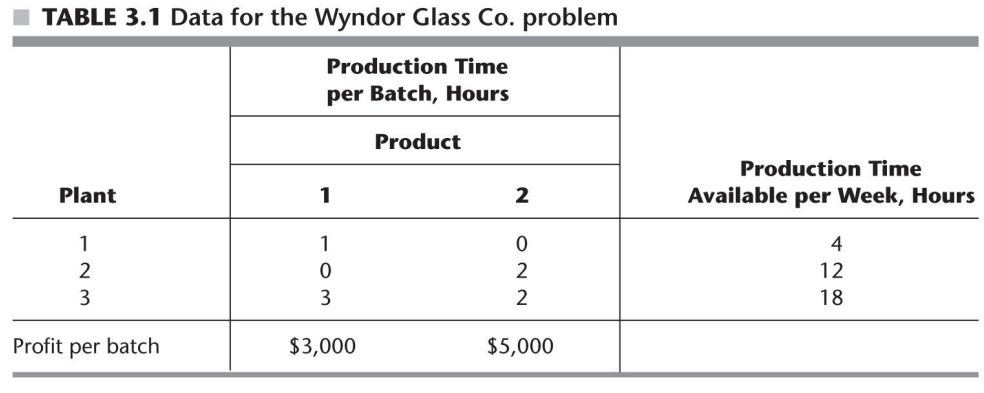
\includegraphics[scale=0.75]{images/lecture1_example1.PNG}
\end{figure}

\noindent
The Wyndor Glass company produces two products; product 1 and product 2.
Product 1 earns a profit of $\$3000$, product 2 earns a profit of $\$5000$.
Before the products can be sold, they first need to pass through 3 processing plants.
Product 1 needs to be processed for 1 hour in plant 1, 0 hours in plant 2 and 3 hours in plant 3.
Likewise, product 2 needs to be processed 0 hours in plant 1, 2 hours in plant 2 and 2 hours in plant 3.
Each processing plant has a limited production time available per week.
Plant 1 can only be active 4 hours per week, plant 2 12 hours per week and plant 3 18 hours per week.
Find an optimal balance between product 1 and product 2 that earns the maximum profit.

\newpage
\noindent
This can be modelled into a linear programming problem as follows:

\begin{align*}
    &\mathrm{max} \quad 3000x_1 + 5000x_2  \\[2pt]
    &\mathrm{s.t.} \quad 
    \begin{array}[t]{r c r c r}
        &  & x_1 & \leq & 4 \\
        &  & 2x_2 & \leq & 12 \\
        3x_1 & + & 2x_2 & \leq & 18       
     \end{array}\\
     &\mathrm{and} \quad x_1, x_2 \geq 0
\end{align*}

\noindent
Where $x_1$ is the amount of product 1 produced per week and $x_2$ is the amount of product 2 produced per week.
Keep in mind all these constraints have to be \textbf{linear} (i.e. no $x_1 \cdot x_2$, $|x|$, $x^2$, etc.).

\noindent
\\
The space in which all constraints are satisfied is called the \textbf{feasible region}:

\begin{figure}[h]
    \centering
    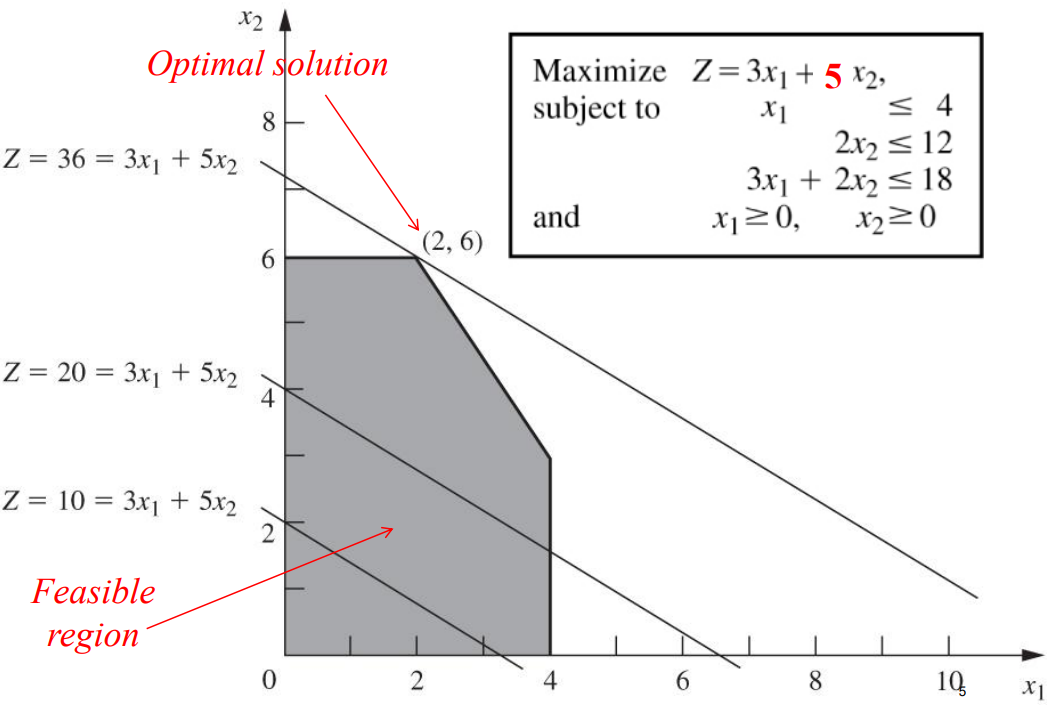
\includegraphics[scale=0.5]{images/lecture1_feasibleregion.PNG}
\end{figure}

\noindent
In some cases, this feasible region is empty. 
If this is the case we say we have an \textbf{infeasible program}.
In the case that the feasible region stretches off to infinity, we say we have an \textbf{unbounded program}.
Note that an unbounded program can still have a bounded optimal solution.

%
% Lecture 2
%
\section*{Lecture 2 - Modelling}
A linear program is \textit{any} program that can be written as maximizing $f(x)$, subject to $Ax \leq b$.
This allows us to model the following relations as well:

\begin{itemize}
    \item $\geq$: $f(x) \geq b \longrightarrow -f(x) \leq -b$
    \item $=$: $f(x) = b \longrightarrow f(x) \leq b \wedge f(x) \geq b$
    \item minimizing: min $f(x)$ $\longrightarrow$ max $-f(x)$
\end{itemize}

\newpage
\noindent
A linear program has a \textbf{standard form}:

\begin{itemize}
    \item Maximization
    \item All functional constraints are in the form $\leq$
    \item Non-negativity constraints on all decision variables
\end{itemize}

\noindent
For modelling questions (i.e. convert a real-world situation into a linear program) you do \textit{not} need to answer in the standard form.
Any answer is fine as long as it is clearly a linear program.

\noindent
\\
Example:

\begin{figure}[h]
    \centering
    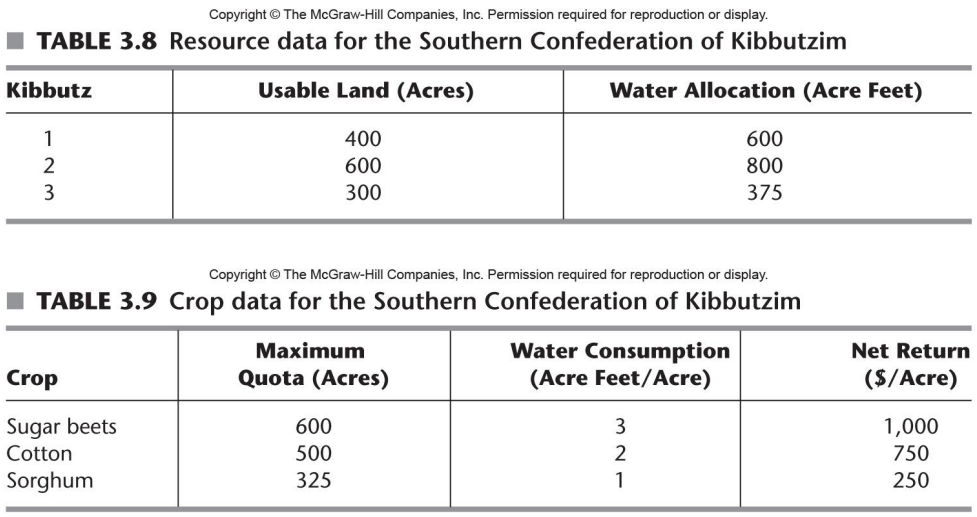
\includegraphics[scale=0.75]{images/lecture2_example1.PNG}
\end{figure}

\noindent
There are 3 farms.
Each farm has a certain amount of usable land in acres, and a maximum number of water allocation for that land.
There are 3 types of crop.
Each type of crop has a certain amount of water consumption per unit, and a profit value.
There is also a maximum amount of each crop available, shared across all 3 farms.
Furthermore, each farm must use the same proportion of its land.
Decide what crops to grow on which farm to maximize the profit across all 3 farms.

\noindent
\\
We can write down the decision variables for this problem as follows:

\begin{table}[h]
    \centering
    \begin{tabular}{l|ccc}
     & \multicolumn{1}{l}{Farm 1} & \multicolumn{1}{l}{Farm 2} & \multicolumn{1}{l}{Farm 3} \\ \hline
    Sugar beets & $x_1$ & $x_2$ & $x_3$ \\
    Cotton & $x_4$ & $x_5$ & $x_6$ \\
    Sorghum & $x_7$ & $x_8$ & $x_9$
    \end{tabular}
\end{table}

\noindent
The problem then becomes to maximize the following equation:

\[ 1000(x_1 + x_2 + x_3) + 750(x_4 + x_5 + x_6) + 250(x_7 + x_8 + x_9) \]

\noindent
Such that:

\newpage
\noindent
\[ x_1 + x_4 + x_7 \leq 400 \]
\[ x_2 + x_5 + x_8 \leq 600 \]
\[ x_3 + x_6 + x_9 \leq 300 \]
\[ \text{acre limits} \]

\[ 3x_1 + 2x_4 + x_7 \leq 600 \]
\[ 3x_2 + 2x_5 + x_8 \leq 800 \]
\[ 3x_3 + 2x_5 + x_9 \leq 375 \]
\[ \text{max. water} \]

\[ x_1 + x_2 + x_3 \leq 600 \]
\[ x_4 + x_5 + x_6 \leq 500 \]
\[ x_7 + x_8 + x_9 \leq 325 \]
\[ \text{max. crop} \]

\[ \frac{x_1 + x_4 + x_7}{400} = \frac{x_2 + x_5 + x_8}{600} = \frac{x_3 + x_6 + x_9}{300} \]
\[ \text{same proportion} \]

\[ x_1, ... , x_9 \geq 0 \]
\[ \text{non-negativity} \]

\noindent
Solving this linear problem leads to the following solution:

\begin{table}[h]
    \centering
    \begin{tabular}{l|ccc}
     & \multicolumn{1}{l}{Farm 1} & \multicolumn{1}{l}{Farm 2} & \multicolumn{1}{l}{Farm 3} \\ \hline
    Sugar beets & $133 \frac{1}{3}$ & $100$ & $25$ \\
    Cotton & $100$ & $250$ & $150$ \\
    Sorghum & $0$ & $0$ & $0$
    \end{tabular}
\end{table}

\noindent
Note that for farm 1 a fractional amount of sugar beets are grown.
In linear programming it is impossible to force an integral solution.
This is another subject called \textbf{Integral Linear Programming}.
Solving integral linear programming problems is NP-hard, because many classical NP-hard problems can be reduced to it.

%
% Lecture 3
%
\newpage
\section*{Lecture 3 - The Simplex Method}
Suppose we have a set of $m$ equalities with $m$ variables.
This can be represented in the system $Ax = b$.
This system has a unique solution \textbf{iff}:

\begin{itemize}
    \item row-rank($A$) = column-rank($A$) = $m$
    \item All rows of $A$ are linearly independent
    \item All columns of $A$ are linearly independent
    \item $A$ is invertible ($A^{-1}$ exists)
\end{itemize}

\noindent
If these conditions do not hold, then the system is either infeasible (no solution exists) or there exist infinitely many solutions.

\subsection*{Corner Points}
\begin{figure}[h]%
    \centering
    \subfloat[\centering Feasible solutions (CPF). \label{fig:cpf}]{{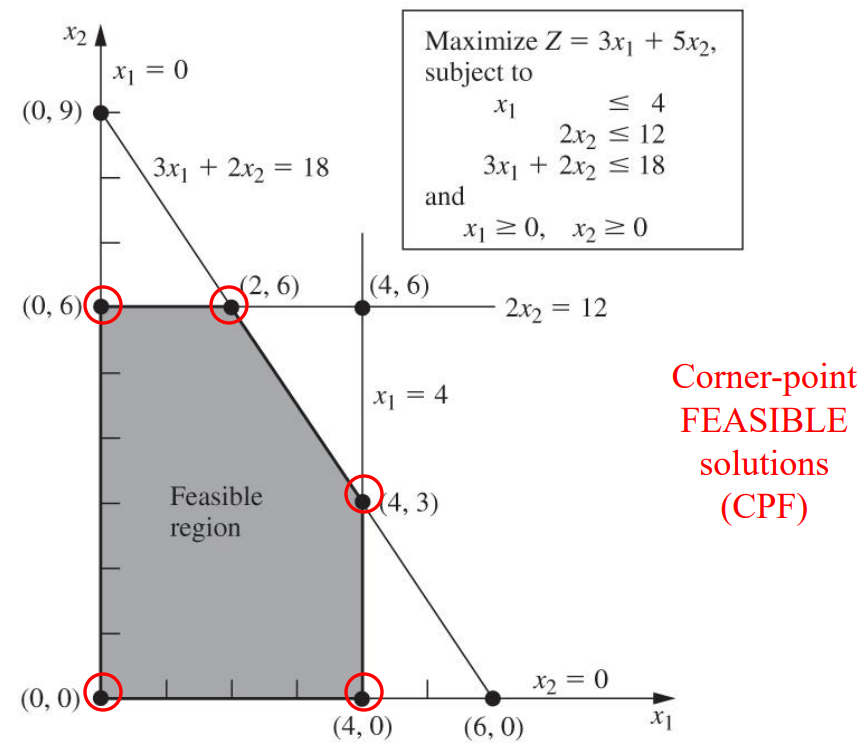
\includegraphics[width=8cm]{images/lecture3_feasiblecornerpointsolutions.PNG}}}%
    \qquad
    \subfloat[\centering Infeasible solutions.]{{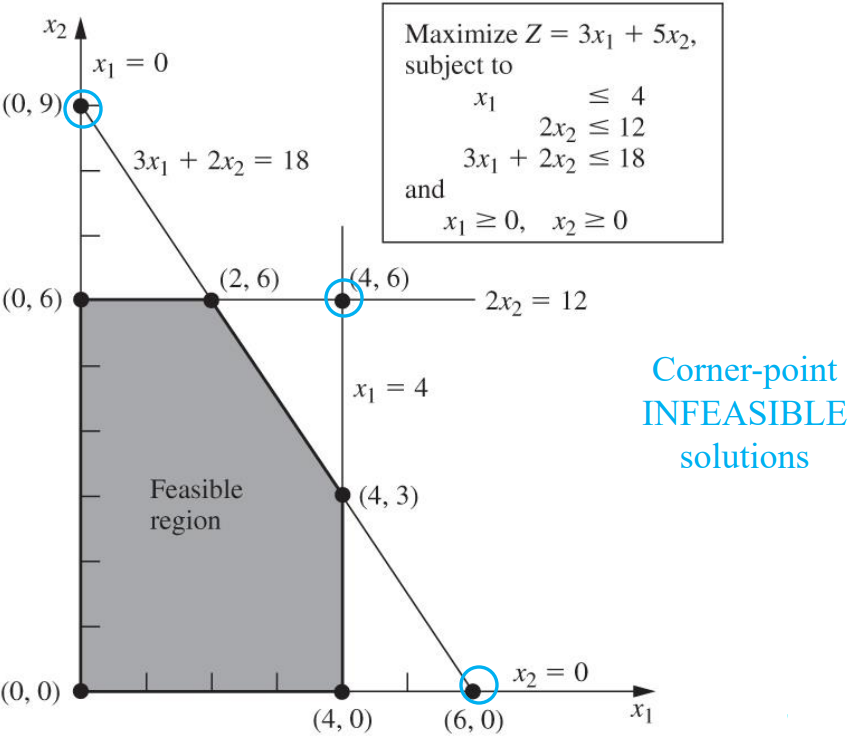
\includegraphics[width=8cm]{images/lecture3_infeasiblecornerpointsolutions.PNG}}}%
    \caption{Corner-point solutions.}%
\end{figure}

\noindent
The Simplex method only considers \textbf{corner-point feasible solutions (CPF)}.

\subsection*{Slack Variables}
Solutions of systems of \textit{inequalities} can be projected to solutions of systems of \textit{equalities} in a higher dimension (i.e. with more variables).
Given the constraint:
\[ x_1 \leq 4 \]

\noindent
With $x_1 \geq 0$. This is equivalent to:
\[ x_1 + x_3 = 4 \]

\noindent
With $x_1, x_3 \geq 0$.
$x_3$ is called a \textbf{slack variable}, because it takes up the slack between $x_1$ and the constraint boundary.
When $x_3 = 0$, $x_1$ is sitting on the constraint (the constraint is \textbf{tight}).

\newpage
\noindent
Using this, we can take our original LP:

\begin{align*}
    &\mathrm{max} \quad 3x_1 + 5x_2  \\[2pt]
    &\mathrm{s.t.} \quad 
    \begin{array}[t]{r c r c r}
        x_1 & & & \leq & 4 \\
        &  & 2x_2 & \leq & 12 \\
        3x_1 & + & 2x_2 & \leq & 18
    \end{array}\\
    &\mathrm{and} \quad x_1, x_2 \geq 0
\end{align*}

\noindent
And transform it to an equivalent, \textbf{augmented form}, LP:

\begin{align*}
    &\mathrm{max} \quad 3x_1 + 5x_2  \\[2pt]
    &\mathrm{s.t.} \quad 
    \begin{array}[t]{r c r c r c r c r c r}
        x_1 & & & + & \textcolor{red}{x_3} & & & & & = & 4 \\
        & & 2x_2 & & & + & \textcolor{red}{x_4} & & & = & 12 \\
        3x_1 & + & 2x_2 & & & & & + & \textcolor{red}{x_5} & = & 18
    \end{array}\\
    &\mathrm{and} \quad x_1, x_2, \textcolor{red}{x_3}, \textcolor{red}{x_4}, \textcolor{red}{x_5} \geq 0
\end{align*}

\noindent
We can also write this in tabular form:

\begin{table}[h]
    \centering
    \begin{tabular}{lllll}
    $x_1$ & $x_2$ & $x_3$ & $x_4$ & $x_5$ \\ \hline
    1 & 0 & 1 & 0 & 0 \\
    0 & 2 & 0 & 1 & 0 \\
    3 & 2 & 0 & 0 & 1
    \end{tabular}
\end{table}

\noindent
Note that because of the 0-1 pattern created by the slack variables, all the rows are linearly independent of each other.
As a result of this the matrix has a row-rank and a column-rank of 3.
This means there exist subsets of 3 columns that are linearly independent of each other (not \textit{every} subset!).
\textbf{These subsets are in a many-to-1 relation related to corner point solutions.}
Example:

\noindent
\\
Take the 3 columns $\{ x_2, x_3, x_5 \}$, and set the remaining columns to 0:

\begin{table}[h]
    \centering
    \begin{tabular}{lllll}
    & $x_2$ & $x_3$ & & $x_5$ \\ \hline
    & 0 & 1 & & 0 \\
    & 2 & 0 & & 0 \\
    & 2 & 0 & & 1
    \end{tabular}
\end{table}

\noindent
If we set this equal to $b$ we get:

\begin{align*}
    \begin{bmatrix}
        0 & 1 & 0 \\
        2 & 0 & 0 \\
        2 & 0 & 1
    \end{bmatrix}
    & = 
    \begin{bmatrix}
        4 \\
        12 \\
        18
    \end{bmatrix}
\end{align*}

\newpage
\noindent
If we solve for $\{ x_2, x_3, x_5 \}$ we get the following answer:

\[ \{ x_1, \textcolor{blue}{x_2}, \textcolor{blue}{x_3}, x_4, \textcolor{blue}{x_5} \} = \{ 0, 6, 4, 0, 6 \} \]

\noindent
If we take $(x_1, x_2)$ from this solution as $(0, 6)$, we can see in figure \ref{fig:cpf} that this corresponds to the corner point on the top left of the feasible region.

\noindent
\\
This solution is called a \textbf{basic solution}.\\
Because the solution is feasible for the LP, it is called a \textbf{basic feasible solution (BFS)}.\\
The \textbf{basis} is $\{ x_2, x_3, x_5 \}$, which are called \textbf{basic variables}.\\
The variables $x_1$ and $x_4$ are called \textbf{nonbasic variables}.\\
Every linearly independent subset of 3 columns is a basis and generates a basic solution, although not all will be feasible:\\
\textbf{A basic solution is feasible iff all variables are non-negative}.

\subsection*{Adjacency}
Two CPF $A$ and $B$ are \textbf{adjacent} iff the two sets of nonbasic variables defining $A$ and $B$ differ in exactly 1 variable.
The variable that is nonbasic in $A$, but basic in $B$ is called the \textbf{entering variable}.
The variable that is basic in $A$, but nonbasic in $B$ is called the \textbf{leaving variable}.

\subsection*{General Principles Behind The Simplex Method}

\begin{itemize}
    \item The Simplex method moves repeatedly from a CPF/BFS to an adjacent CPF/BFS.
    \item If it can, it starts at the origin (e.g. in the above example BFS $(0, 0, 4, 12, 18)$).
    \item It is 'greedy', in the sense that it \textit{never} moves to an adjacent CPF/BFS that lowers the objective function.
    \item A CPF/BFS is optimal iff none of its adjacent neighbors improve the objective function.
\end{itemize}

\subsection*{Solving Problems With The Simplex Method}
For convenience, the Simplex method treats the current value of the object function ($Z$) as another variable:
\begin{align*}
    &\mathrm{max} \quad Z \\[2pt]
    &\mathrm{s.t.} \quad 
    \begin{array}[t]{c r c r c r c r c r c r c r}
        (0) & Z & - & 3x_1 & - & 5x_2 & & & & & & & = & 0 \\
        (1) & & & x_1 & & & + & x_3 & & & & & = & 4 \\
        (2) & & & & & 2x_2 & & & + & x_4 & & & = & 12 \\
        (3) & & & 3x_1 & + & 2x_2 & & & & & + & x_5 & = & 18
    \end{array}\\
    &\mathrm{and} \quad x_j \geq 0
\end{align*}

\noindent
At the beginning we take $\{ x_3, x_4, x_5 \}$ as the basis, because this means $x_1$, $x_2$ and $Z$ start off as 0 (i.e. the program starts at the origin).
Note that \textbf{basic variables do not appear in the objective function}.
The Simplex method makes sure this will never be the case.

\newpage
\noindent
To pick our entering variable, look at the objective function and see which nonbasic variable has the biggest \textbf{per-unit increase}:
\[ \text{Change in } Z \text{ per unit increase } x_1 : 3 \]
\[ \text{Change in } Z \text{ per unit increase } x_2 : 5 \]

\noindent
So $x_2$ will become the entering variable.
To see which basic variable becomes the leaving variable, we rewrite the equations in terms of $\{ x_3, x_4, x_5 \}$:
\begin{align*}
    \begin{array}[t]{c r c r c}
        x_3 & = & 4 & & \\
        x_4 & = & 12 & - & 2x_2 \\
        x_5 & = & 18 & - & 2x_2
    \end{array}
\end{align*}

\noindent
Keep in mind $x_1$ doesn't show up because it stays nonbasic (i.e. $x_1 = 0$).
Note that $x_3$ is not changed by an increase in $x_2$, because the system is already tight with its decision boundary.
To see which basic variable reaches 0 first we can use the \textbf{minimum ratio test}:
$\frac{12}{2} < \frac{18}{2}$, thus $x_4$ will be the leaving variable.

\noindent
\\
To update the system we use \textbf{Gaussian elimination}.
We need to rewrite the \textit{column} of the entering variable ($x_2$), such that it has coefficients of 0 everywhere except the \textit{row} of the leaving variable ($x_4$).
This has the effect of removing $x_2$ from the objective function, while adding $x_4$:
\begin{align*}
    &\mathrm{max} \quad Z \\[2pt]
    &\mathrm{s.t.} \quad 
    \begin{array}[t]{c r c r c r c r c r c r c r}
        (0) & Z & - & 3x_1 & & & & & + & \frac{5}{2}x_4 & & & = & 30 \\
        (1) & & & x_1 & & & + & x_3 & & & & & = & 4 \\
        (2) & & & & & x_2 & & & + & \frac{1}{2}x_4 & & & = & 6 \\
        (3) & & & 3x_1 & & & & & - & x_4 & + & x_5 & = & 6
    \end{array}\\
    &\mathrm{and} \quad x_j \geq 0
\end{align*}

\noindent
The new basis is $\{ x_2, x_3, x_5 \}$, $(x_1, x_2, x_3, x_4, x_5) = (0, 6, 4, 0, 6)$ and the new value of the objective function is $Z = 30$.

\noindent
\\
We are not done yet, as the objective function still contains a negative coefficient (i.e. $x_1$ still has potential to improve $Z$, while the positive coefficient of $x_4$ means that increasing it \textit{cannot} improve $Z$ any further).
This means $x_1$ will be our entering variable, and we can find our leaving variable by doing the minimum ratio test again:
\begin{align*}
    \begin{array}[t]{c r c r c}
        x_3 & = & 4 & - & x_1 \\
        x_2 & = & 6 & & \\
        x_5 & = & 6 & - & 3x_1
    \end{array}
\end{align*}

\noindent
$\frac{6}{3} < \frac{4}{1}$, so $x_5$ will be the leaving variable.

\newpage
\noindent
By applying Gaussian elimination again we can reach the following system:
\begin{align*}
    &\mathrm{max} \quad Z \\[2pt]
    &\mathrm{s.t.} \quad 
    \begin{array}[t]{c r c r c r c r c r c r c r}
        (0) & Z & & & & & & & + & \frac{3}{2}x_4 & + & x_5 & = & 36 \\
        (1) & & & & & & & x_3 & + & \frac{1}{3}x_4 & - & \frac{1}{3}x_5 & = & 2 \\
        (2) & & & & & x_2 & & & + & \frac{1}{2}x_4 & & & = & 6 \\
        (3) & & & x_1 & & & & & - & \frac{1}{3}x_4 & + & \frac{1}{3}x_5 & = & 2
    \end{array}\\
    &\mathrm{and} \quad x_j \geq 0
\end{align*}

\noindent
The new basis is $\{ x_1, x_2, x_3 \}$, $(x_1, x_2, x_3, x_4, x_5) = (2, 6, 2, 0, 0)$ and the new value of the objective function is $Z = 36$.

\noindent
\\
We are done, since none of the two nonbasic variables can improve the objective function $Z$ any further.
This means we have reached optimality.

\begin{figure}[h]
    \centering
    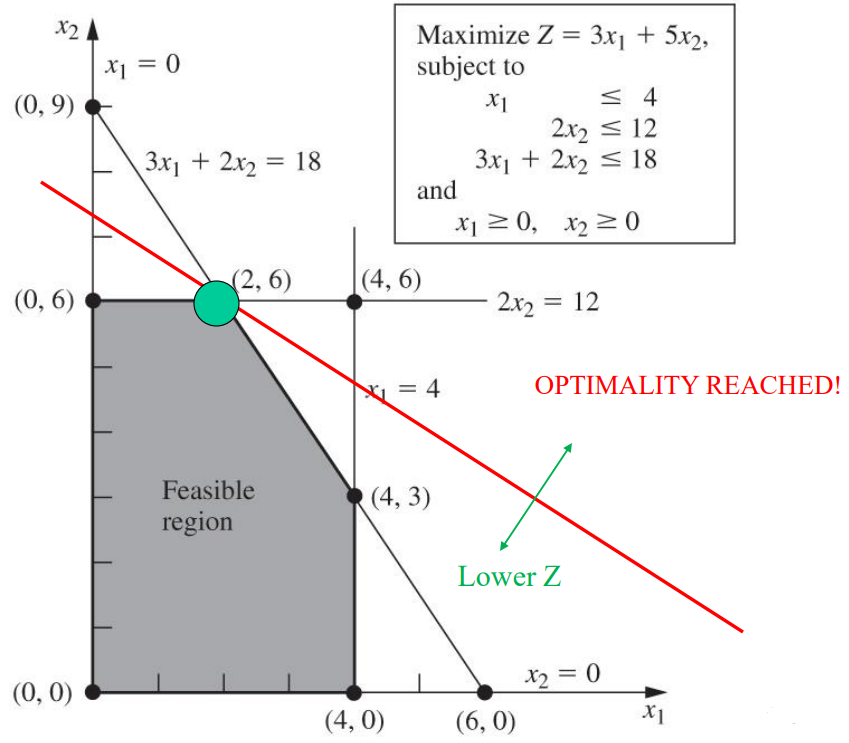
\includegraphics[scale=0.6]{images/lecture3_finalsolution.PNG}
\end{figure}

\noindent
\textbf{The complete process:}

\begin{enumerate}
    \item Can a nonbasic variable improve the objective function?
    \item If no, then we are done.
    \item If yes, find the nonbasic variable with the most potential to improve the objective function, this will be the entering variable.
    \item Use the minimum ratio test to identify the leaving variable.
    \item Update the system for the new BFS using Gaussian elimination.
    \item Go back to step 1.
\end{enumerate}

%
% Lecture 4
%
\newpage
\section*{Lecture 4 - The Simplex Tableau}
We earlier stated that, without sacrificing generality, we can assume every linear program is written in the form:

\begin{enumerate}
    \item Maximization
    \item All constraints are $\leq$
    \item All decision variables are non-negative
\end{enumerate}

\noindent
We can also make a 4th assumption: \textbf{The RHS of the $\leq$ constraints are non-negative}.
This assumption can't be made without loss of generality (e.g. how to model $x \geq 5$?), but is useful because it means the origin is \textit{always} a feasible solution.
For now, just assume these 4 assumptions hold for every linear program.

\noindent
\\
How to solve the previously discussed example using a Simplex tableau:

\begin{figure}[h]
    \centering
    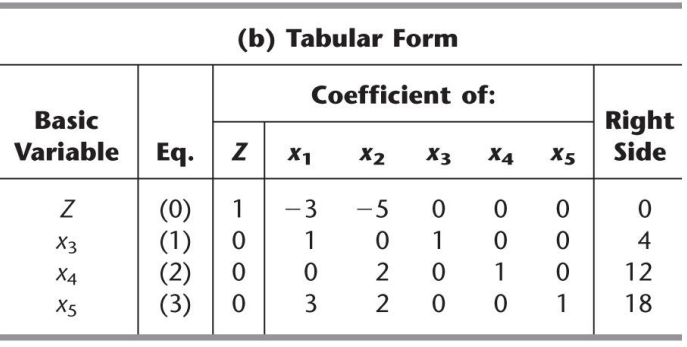
\includegraphics[scale=0.75]{images/lecture4_table1.PNG}
\end{figure}

\begin{figure}[h]
    \centering
    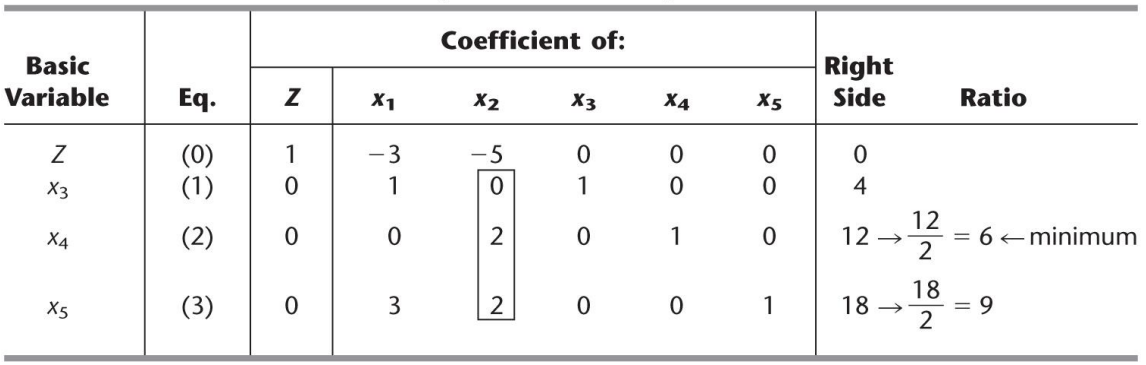
\includegraphics[scale=0.65]{images/lecture4_table2.PNG}
    \caption{Determining the first leaving variable using the minimum ratio test. We say $x_2$ is the \textbf{pivot column} and equation (2) is the \textbf{pivoting row}.}
\end{figure}

\newpage
\begin{figure}[h]
    \centering
    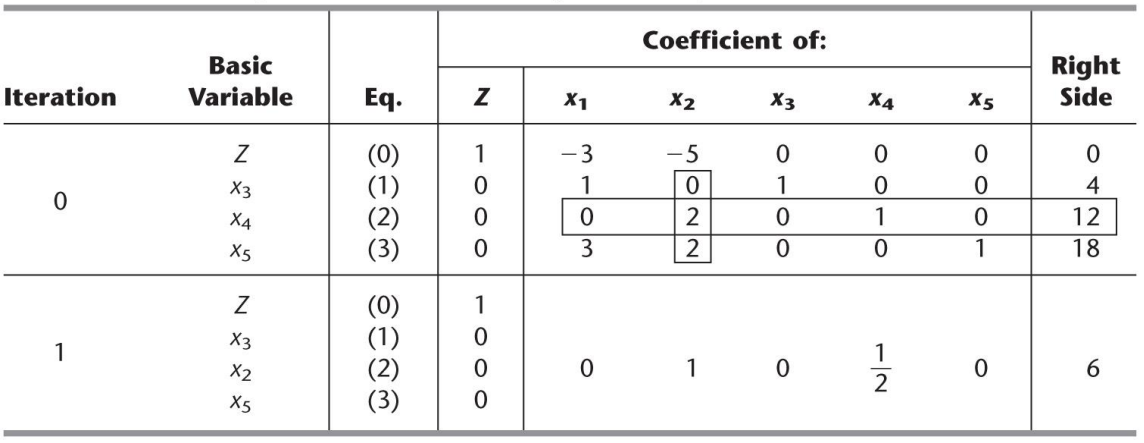
\includegraphics[scale=0.6]{images/lecture4_table3.PNG}
    \caption{Dividing the pivot row by the pivot number.}
\end{figure}

\begin{figure}[h]
    \centering
    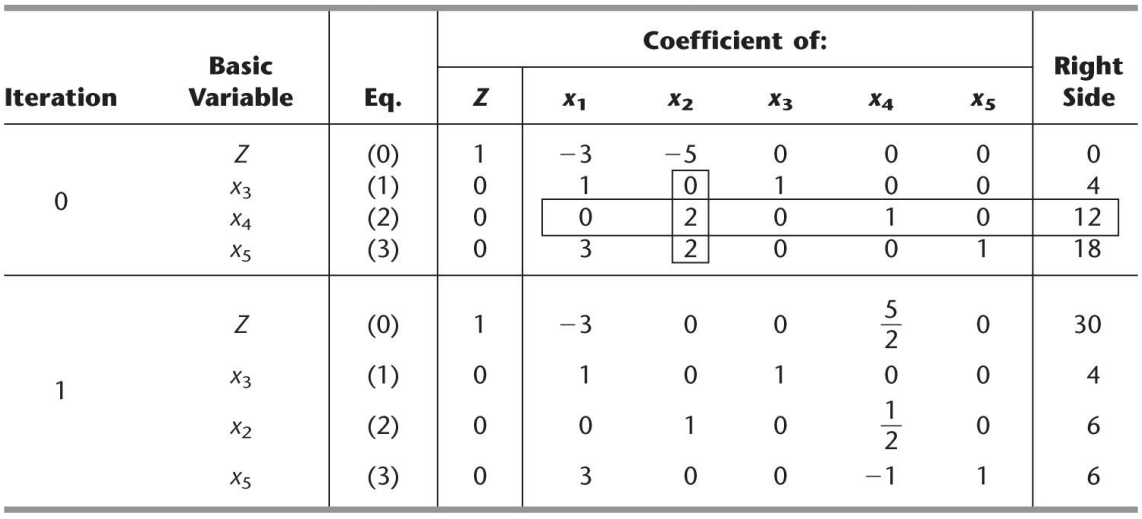
\includegraphics[scale=0.6]{images/lecture4_table4.PNG}
    \caption{The tableau after the first iteration of the Simplex method.}
\end{figure}

\begin{figure}[h!]
    \centering
    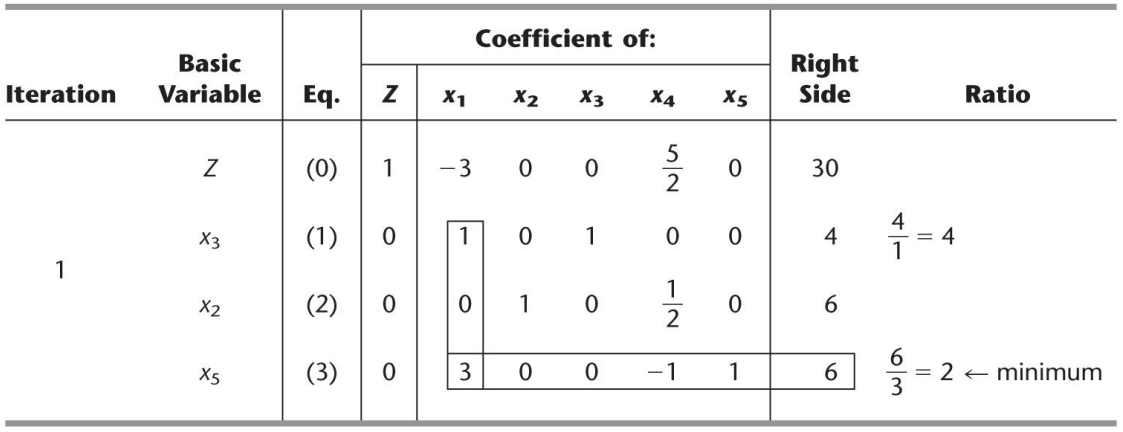
\includegraphics[scale=0.6]{images/lecture4_table5.PNG}
    \caption{Determining the second leaving variable using the minimum ratio test.}
\end{figure}

\newpage
\begin{figure}[h]
    \centering
    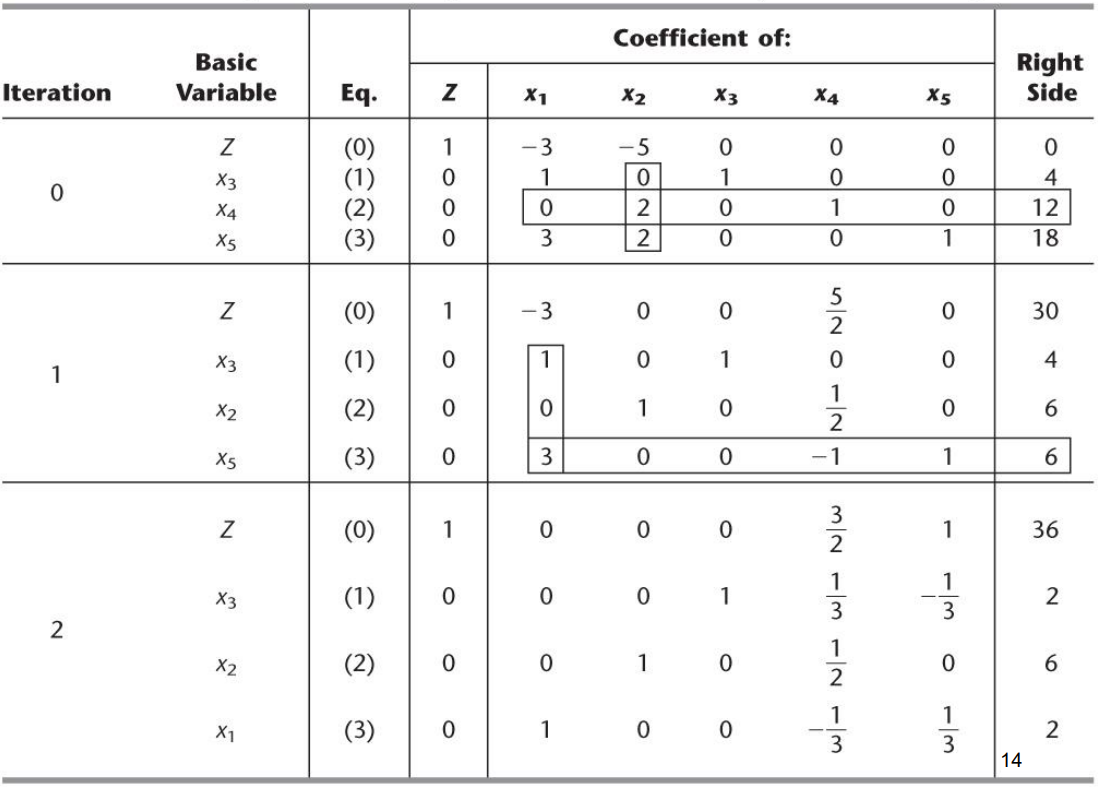
\includegraphics[scale=0.7]{images/lecture4_table6.PNG}
    \caption{The final tableau.}
\end{figure}

\subsection*{Pivoting Rules}

\begin{itemize}
    \item \textbf{What if there is no leaving variable?} (i.e. all the numbers in the column of the entering variable are $\leq 0$) This is a sign that the LP is \textbf{unbounded}.
    \item \textbf{What if there is a tie for the entering / leaving variable?} (i.e. a tie for negative value in the top row, or tie for the minimum ratio test) The short answer is to just break ties arbitrarily, the long answer has to do with \textbf{degeneracy}.
\end{itemize}

\subsection*{Degeneracy}
A BFS is degenerate if one or more of its basic variables is 0.
Such a variable is called a \textbf{degenerate basic variable}.
The core of degeneracy is that in an $n$-dimensional system you need at least $n$ tight constraint boundaries to define a point, but there can be more (e.g. think the tip of a diamond in 3-dimensions).
If a CPF/BFS has more than $n$ constraint boundaries tight, then this CPF/BFS is called a \textbf{degenerate CPF/BFS}.
The consequence of this is that the Simplex method sometimes goes from corner point to corner point without increasing the objective function (i.e. it is stuck in the same BFS).
This is called \textbf{stalling} and only happens in very specific circumstances.
If it gets stuck in a loop forever it is called \textbf{cycling}, but it is proven that, using special rules, you can make the Simplex method always terminate.

%
% Lecture 5
%
\newpage
\section*{Lecture 5 - Adapting Models}
So far we have looked at linear programs that are in the standard form and also have an additional constraint:

\begin{itemize}
    \item The RHS of all $\leq$ constraints are non-negative.
\end{itemize}

\noindent
This makes it easier to find an initial BFS (the origin), but not every linear program will be in this form.
For example, we can code up an $=$ constraint as two $\leq$ constraints (e.g. $x = 3 \Leftrightarrow x \leq 3$ and $-x \leq -3$), but this only shifts the problem elsewhere.

\subsection*{Big-M Method}
We can deal with $=$ constraints using \textbf{artificial variables}.
For example, we can turn the constraint $3x_1 + 2x_2 = 18$ into:
\[ 3x_1 + 2x_2 + \textcolor{red}{x_3} = 18 \]

\noindent
Where $\textcolor{red}{x_3}$ is an artificial variable.
This variable allows the constraint to be violated, essentially turning the $=$ constraint into a $\leq$ constraint.
We do this to turn the constraint into the friendly '$\leq$ non-negative' form which we know how to deal with (if the RHS is negative to begin with, multiply the entire constraint by -1).

\noindent
\\
To discourage the LP from violating this constraint, we assign a massive negative penalty to the artificial variables:
\[ \max Z = 3x_1 + 5x_2 - \textcolor{red}{Mx_5} \]

\noindent
Here $\textcolor{red}{M}$ is simply a 'very large number'.
Think of it as an infinity.

\noindent
\\
Because $M$ is such a large number, the LP will prioritize getting rid of it in the Simplex tableau.
After sufficiently many pivots the $M$ term will disappear from the value of the objective function.
This means the LP has now entered the feasible region, as the constraints with artificial variables are no longer being violated (see example).

\noindent
\\
Next up is how we deal with $\geq$ constraints.
$\geq$ constraints with a negative RHS can be converted to '$\leq$ non-negative' form by multiplying the entire constraint by -1, but $\geq$ constraints with a positive RHS are a problem.
We can solve this by using an idea similar to slack variables, called \textbf{surplus variables}.

\noindent
\\
Given the constraint $2x_1 + 3x_2 \geq 5$, we can convert it into an $=$ constraint using a surplus variable:
\[ 2x_1 + 3x_2 - \textcolor{blue}{x_3} = 5 \]

\noindent
The surplus variable here is $\textcolor{blue}{x_3}$, and measures the distance \textit{above} the constraint boundary (as opposed to \textit{below} the constraint boundary, which slack variables do).
To finish this example, simply add an artificial variable to the constraint as follows:
\[ 2x_1 + 3x_2 - \textcolor{blue}{x_3} + \textcolor{red}{x_4} = 5 \]

\newpage
\begin{figure}[h]
    \centering
    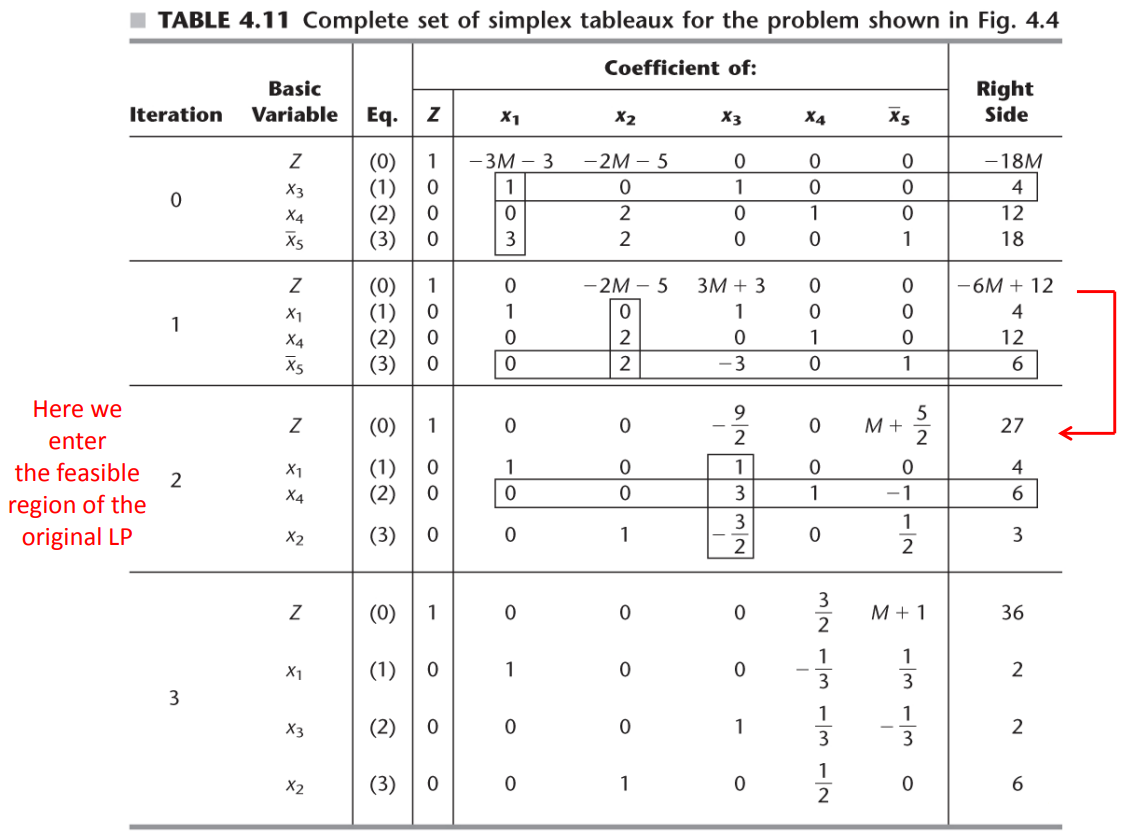
\includegraphics[scale=0.65]{images/lecture5_bigmtableau.PNG}
    \caption{An example of the big-M method.}
\end{figure}

\begin{figure}[h!]
    \centering
    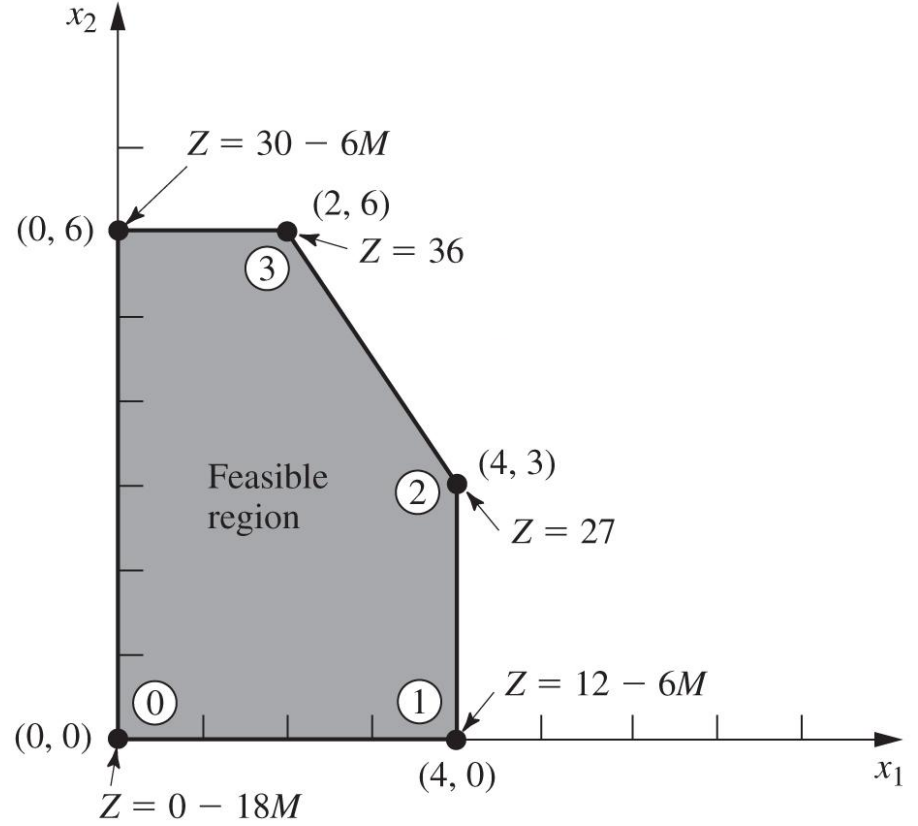
\includegraphics[scale=0.6]{images/lecture5_bigmfeasibleregion.PNG}
\end{figure}

\newpage
\noindent
Because the Simplex method chooses the most negative number in the top row, it will always start by removing all the $M$ instances.
The whole process is kind of divided into 2 phases:

\begin{enumerate}
    \item \underline{Entering} the feasible region.
    \item \underline{Optimizing} within the feasible region.
\end{enumerate}

\subsection*{Two-Phase Method}
The two-phase method solves two problems:

\begin{enumerate}
    \item Minimize the sum of the artificial variables, subject to revised constraints. The optimal solution obtained for this problem (with $Z = 0$) will be a BFS for the real problem.
    \item Find the optimal solution for the real problem, starting from the BFS obtained in step 1. Since the artificial variables are not part of the real problem, they can be dropped (they are all zero now anyway).
\end{enumerate}

\subsection*{Augmented Forms}
\begin{figure}[h]
    \centering
    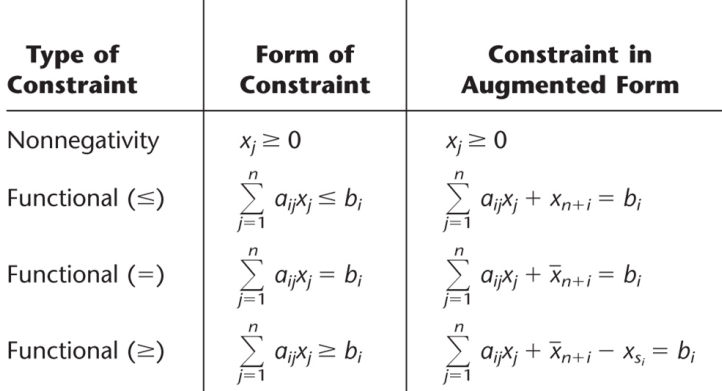
\includegraphics[scale=0.75]{images/lecture5_augmentedform.PNG}
\end{figure}

\noindent
The last thing to consider is what if we don't want non-negativity constraints on the decision variables?
We can deal with this using substitution:

\begin{itemize}
    \item \textbf{Case 1:} a decision variable has a different range (e.g. $x_1 \geq -10$). Let $x_1^\prime = x_1 + 10$, $x_1^\prime \geq 0$. We can solve this case by substituting $(x_1^\prime - 10)$ for every $x_1$ in the LP.
    \item \textbf{Case 2:} a decision variable is completely unconstrained. Let $x_1 = x_1^+ - x_1^-$, with $x_1^+, x_1^- \geq 0$. We can solve this case by substituting $x_1^+ - x_1^-$ for every $x_1$ in the LP.
\end{itemize}

%
% Lecture 6
%
\newpage
\section*{Lecture 6 - Intro to Post-Optimality Analysis}
After solving an LP, suppose someone asks you to re-solve the LP with slightly changed coefficients.
You could just re-solve it from the beginning, but this is really inefficient for large LP problems.

\subsection*{Shadow Prices}
Suppose someone wants to slightly change the RHS of the functional constraints.
If these changes are not \textit{'too big'} (will be defined later), then the same basis will still be optimal.
The location of the corresponding BFS might differ, but the same set of constraints will be tight.
Deriving the new solution / BFS is a lot easier than re-executing the Simplex method.

\begin{figure}[h]
    \centering
    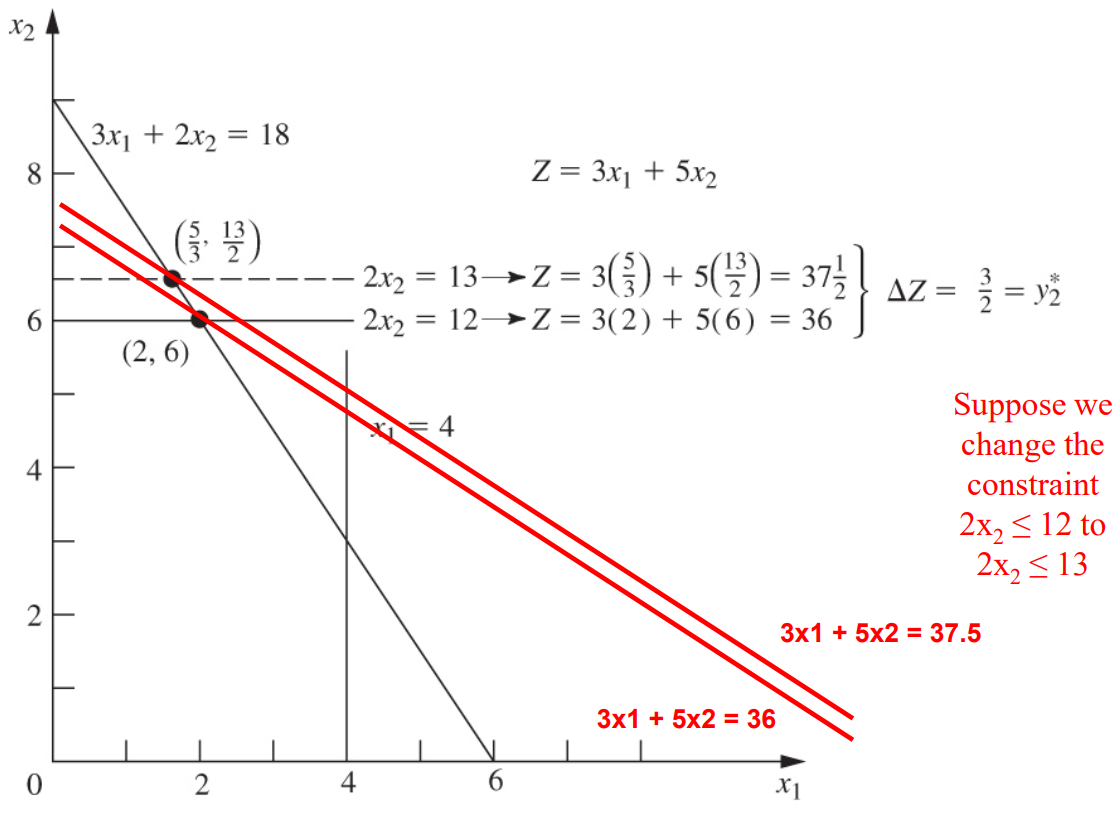
\includegraphics[scale=0.5]{images/lecture6_shadowprices1.PNG}
    \caption{Note that the same basis is optimal.}
\end{figure}

\begin{figure}[h!]
    \centering
    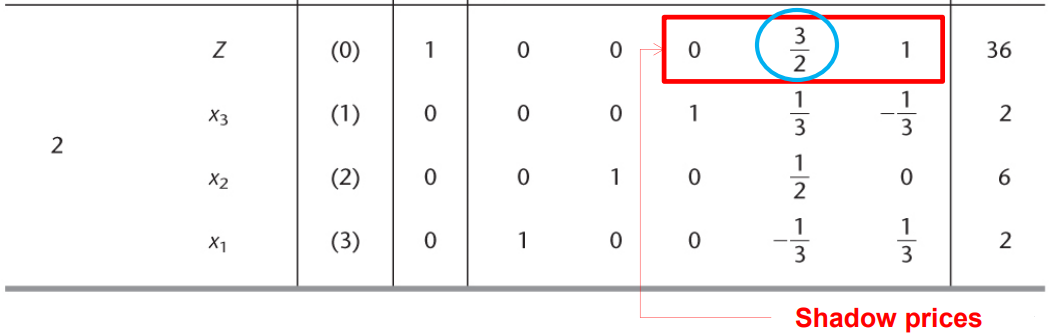
\includegraphics[scale=0.5]{images/lecture6_shadowprices2.PNG}
    \caption{The per-unit change for slack variable $x_4$ is 1.5.}
\end{figure}

\noindent
The coefficients of the slack variables in the top row of the final simplex tableau tell you how the optimum changes for a unit change in the right-hand-side of the corresponding constraint.
Note that this only holds if the changes are not \textit{'too big'}.
If you go too far the optimum flips to a different basis.

\newpage
\subsection*{Computer Implementation}
The Simplex method is still the standard algorithm used by many LP solvers, but note there are many specialized implementations of the Simplex method that are superior for solving special types of LP (transport, network, etc.).
With the Simplex method, the number of functional constraints is the most important factor in determining the running time.

\subsection*{Interior-Point Methods}
Interior-point methods go \textit{through} the feasible region, not around the perimeter.
This is faster than the Simplex method for larger LPs:

\begin{itemize}
    \item \textbf{The Simplex method} executes many iterations, each one being performed very quickly.
    \item \textbf{Interior-point methods} require fewer iterations, but each one takes quite a long time.
\end{itemize}

\noindent
If the feasible region has a vast number of CPF solutions, and they do not quickly lead to optimality, interior-point methods will be better.
Interior-point methods do not care about how 'spiky' the outside of the feasible region is.

\noindent
\\
Many LP solvers also include at least one interior-point \textbf{"barrier"} algorithm.
Unfortunately interior-point methods do not provide the same kind of post-optimality analysis as the Simplex method.
A solution to this are \textbf{"cross-over"} algorithms, which get close to optimality using interior-point methods and then try to find a BFS using the Simplex method for the last steps.
This sounds easy but note that finding a BFS near an interior point is not a trivial task.

%
% Lecture 7
%
\section*{Lecture 7 - Convexity}
In linear programming, an important idea is the concept of a \textbf{line segment}:

\noindent
\\
Let $x^\prime$ and $x^{\prime\prime}$ be any two points in the feasible region.
The line segment connecting $x^\prime$ and $x^{\prime\prime}$ is the set of all points that lie on the line connecting $x^\prime$ and $x^{\prime\prime}$.
Any point on this line segment can be written as:
\[ \Delta x^\prime + (1 - \Delta)x^{\prime\prime} \]

\noindent
Where $0 \leq \Delta \leq 1$.

\noindent
\\
In linear programming, every possible feasible region is a \textbf{convex set}:

\begin{figure}[h]
    \centering
    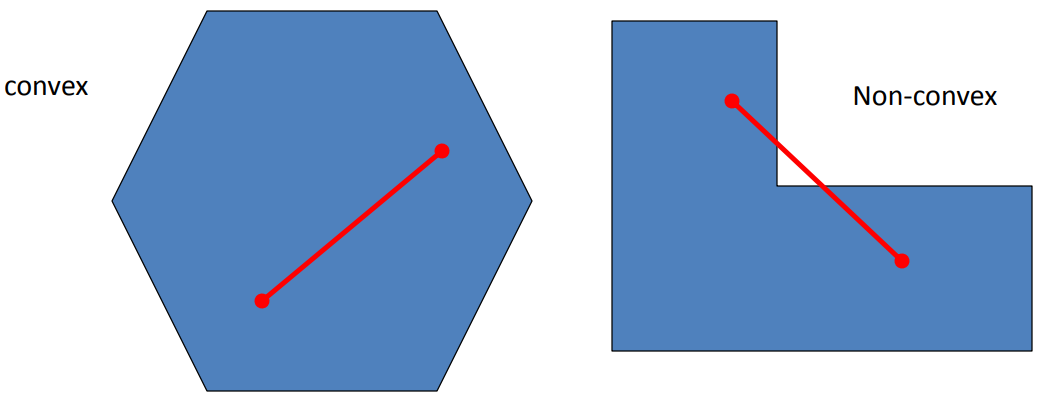
\includegraphics[scale=0.5]{images/lecture7_convexity.PNG}
\end{figure}

\newpage
\noindent
This is also why a constraint like $x_1 \neq 3$ is impossible in linear programming, this would make the feasible region non-convex.

\noindent
\\
If the feasible region is bounded in every direction, then the feasible region is a \textbf{convex polytope}:

\begin{figure}[h]
    \centering
    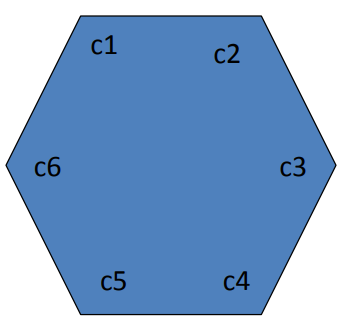
\includegraphics[scale=0.5]{images/lecture7_polytope.PNG}
\end{figure}

\noindent
Every point inside a convex polytope can be written as a \textbf{convex sum} of its corner points.
In the above example it would look like this:
\[ P = \lambda_1c_1 + \lambda_2c_2 + \lambda_3c_3 + \lambda_4c_4 + \lambda_5c_5 + \lambda_6c_6 \]

\noindent
Where $\lambda_1 \geq 0$ and $\lambda_1 + \lambda_2 + \lambda_3 + \lambda_4 + \lambda_5 + \lambda_6 = 1$.

\noindent
\\
The set of optimal solutions of an LP is also a convex polytope (assuming the set is bounded).
This convex polytope is always of lower dimension than the feasible region:

\begin{figure}[h]
    \centering
    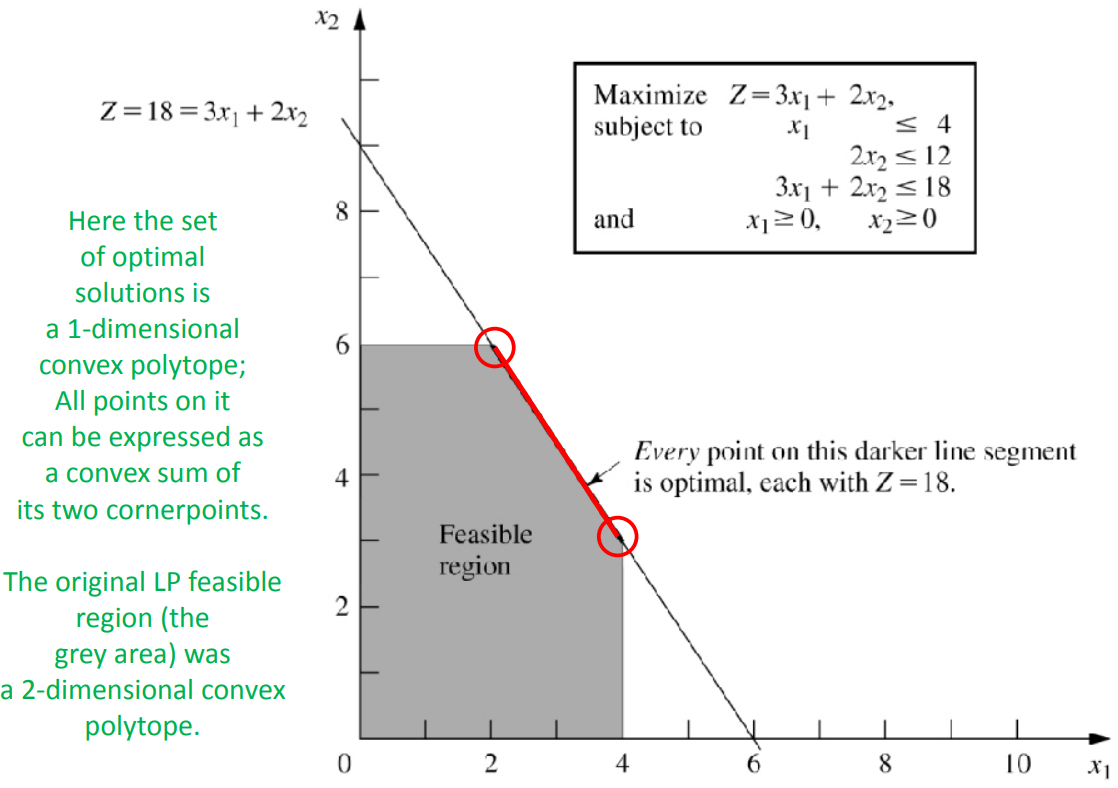
\includegraphics[scale=0.75]{images/lecture7_optimalsolutions_polytope.PNG}
\end{figure}

\newpage
\subsection*{Alternative Definition CPF/BFS}
A corner point feasible solution is any point $x^*$ in the feasible region that does \underline{not} lie on the line segment of two feasible points $x^\prime$ and $x^{\prime\prime}$, where $x^\prime, x^{\prime\prime} \neq x^*$.

\noindent
\\
This definition is useful when constructing proofs, for example:

\noindent
\\
\textbf{Claim:} If there is exactly one optimal solution, it must be a CPF solution.\\
\textbf{Proof:} Assume we are dealing with a maximization LP.
Suppose there is only one optimal solution $x^*$, and it is \textit{not} a CPF solution.
This means it can be written as the convex sum of two points $x^\prime$ and $x^{\prime\prime}$ in the feasible region, where neither point is equal to $x^*$.
We can write this as:
\[ x^* = \Delta x^\prime + (1 - \Delta)x^{\prime\prime} \]

\noindent
Where $0 < \Delta < 1$.
Now, let $Z$ be the value of the objective function associated with $x^*$, and let $Z^\prime$ and $Z^{\prime\prime}$ be the values of the objective function associated with $x^\prime$ and $x^{\prime\prime}$ respectively.
Using linearity, we can write this as:
\[ Z^* = \Delta Z^\prime + (1 - \Delta)Z^{\prime\prime} \]

\noindent
Because we know $Z^*$ is an optimal solution, we also know $Z^\prime \leq Z^*$ and $Z^{\prime\prime} \leq Z^*$.
This gives us two cases:

\begin{itemize}
    \item \textbf{Case 1:} $Z^\prime = Z^*$ or $Z^{\prime\prime} = Z^*$. This means we have more than one optimal solution, which contradicts the original claim.
    \item \textbf{Case 2:} $Z^\prime < Z^*$ and $Z^{\prime\prime} < Z^*$. This means $\Delta Z^\prime + (1 - \Delta)Z^{\prime\prime} < Z^*$, which is also a contradiction.
\end{itemize}

\noindent
This means our initial assumption was wrong, which means the claim is true. $\Box$

\subsection*{Useful Proof Technique}
If you want to prove that a feasible solution $x^*$ to an LP is \underline{not} a BFS, you can write it as the weighted average of two other distinct feasible solutions $x^\prime$ and $x^{\prime\prime}$.

\noindent
\\
Often you do this by adding and subtracting $\epsilon$ from $x^*$ such that these new points are still feasible, and such that $x^*$ lies halfway between them.

%
% Lecture 8
%
\newpage
\section*{Lecture 8 - Algebraic Simplex Tableau}
We will discuss something called the \textbf{matrix form} of the Simplex method.
This forms the basis of the \textbf{revised Simplex method}, which is the algorithm used by most real Simplex implementations because it allows all data to be stored compactly.

\noindent
\\
The \textit{initial} Simplex tableau in matrix form looks like this:

\begin{figure}[h]
    \centering
    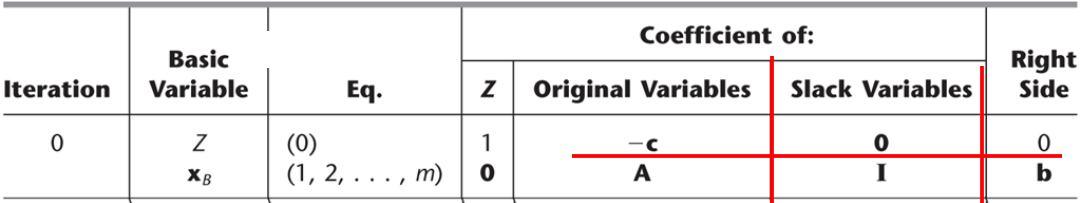
\includegraphics[scale=0.75]{images/lecture8_initialsimplextableau1.PNG}
    \caption{The Simplex tableau in matrix form.}
\end{figure}

\begin{figure}[h]
    \centering
    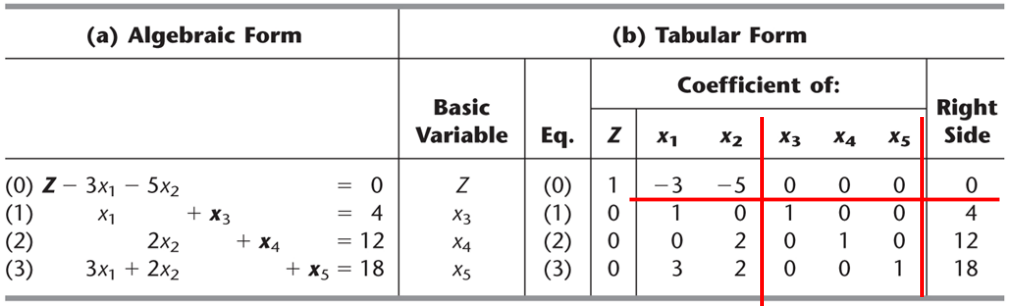
\includegraphics[scale=0.75]{images/lecture8_initialsimplextableau2.PNG}
    \caption{The Simplex tableau in tabular form.}
\end{figure}

\noindent
The matrix form uses the following matrices:

\begin{itemize}
    \item $A$: the constraint matrix ($m \text{ constraints} \times n \text{ decision variables}$)
    \item $b$: 'RHS' (column vector of length $m$)
    \item $c$: coefficients of decision variables in the objective function (row vector of length $n$)
\end{itemize}

\noindent
We can describe the Simplex tableau in matrix form for every possible state of the tableau.
The entire Simplex tableau can be constructed just from knowing the basis.
The basis tells us the following matrices:

\begin{itemize}
    \item $B$: columns of $\left[ A : I \right]$ corresponding to basic variables ($m \times m$ invertible matrix)
    \item $c_B$: coefficients of the basic variables in the objective function
\end{itemize}

\noindent
Furthermore, we can obtain the basic variables as $x_B = B^{-1}b$, and the value of the objective function as $Z = c_B x_B = c_B B^{-1} b$.

\newpage
\begin{figure}[h]
    \centering
    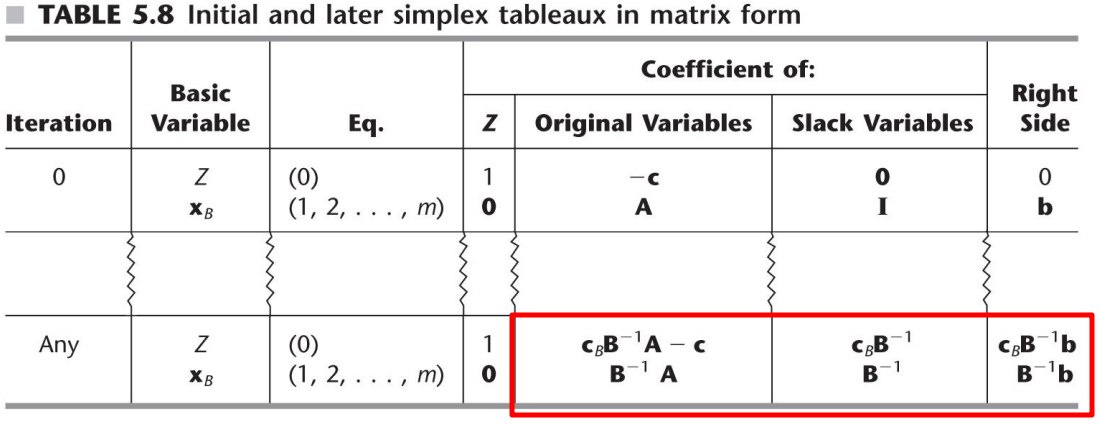
\includegraphics[scale=0.75]{images/lecture8_latersimplextableau.PNG}
\end{figure}

\subsection*{Revised Simplex Method}
Using the matrix form of the Simplex tableau is very space efficient, but it is (initially) not very fast.
Every pivot you have to construct $B^{-1}$ by inverting $B$, which is time-consuming ($O(n^3)$).
The revised Simplex method speeds this up by pivoting \textit{inside} the $B^{-1}$ matrix, which means you don't have to invert it anymore.
This is much faster than inverting $B$ from scratch ($O(n^2)$).
Another advantage is that in LP the $A$ and $B$ matrices are often sparse.
Elementary row operations on sparse matrices can be done very quickly using specialized algorithms.

\noindent
\\
The trouble with dynamically updating $B^{-1}$ is that numerical rounding errors can quickly accumulate because of the row operations.
For this reason actual implementations of the revised Simplex method will occasionally invert $B^{-1}$ from scratch, to get rid of any accumulated rounding errors.

%
% Lecture 9
%
\newpage
\section*{Lecture 9 - Duality}
Take the following linear program:
\begin{align*}
    &\mathrm{max} \quad Z = 3x_1 + 4x_2  \\[2pt]
    &\mathrm{s.t.} \quad 
    \begin{array}[t]{r c r c r}
        x_1 & + & 2x_2 & \leq & 10 \\
        2x_1 & + & 3x_2 & \leq & 15
    \end{array}\\
    &\mathrm{and} \quad x_1, x_2 \geq 0
\end{align*}

\noindent
We know any feasible solution gives a lower bound on the optimum value of $Z$, but what about \textit{upper} bounds?
Suppose we multiply constraint 1 by 3:
\[ 3x_1 + 6x_2 \leq 30 \]

\noindent
This is always greater than or equal to the objective function, which means 30 is an upper bound of $Z$.
If we try adding constraint 1 to constraint 2 we get the following:
\[ 3x_1 + 5x_2 \leq 25 \]

\noindent
This is still greater than or equal to the objective function, which means 25 is an upper bound of $Z$ as well.

\noindent
\\
Suppose we want to systematically determine the best upper bound that this technique can generate for a given LP.
We want a linear sum of the constraints such that this sum is bigger than or equal to the objective function (i.e. is an upper bound), but such that the sum of the RHS is as low as possible.
Let $y_1$ be the multiple we take of constraint 1, and let $y_2$ be the multiple we take of constraint 2:

\begin{figure}[h]
    \centering
    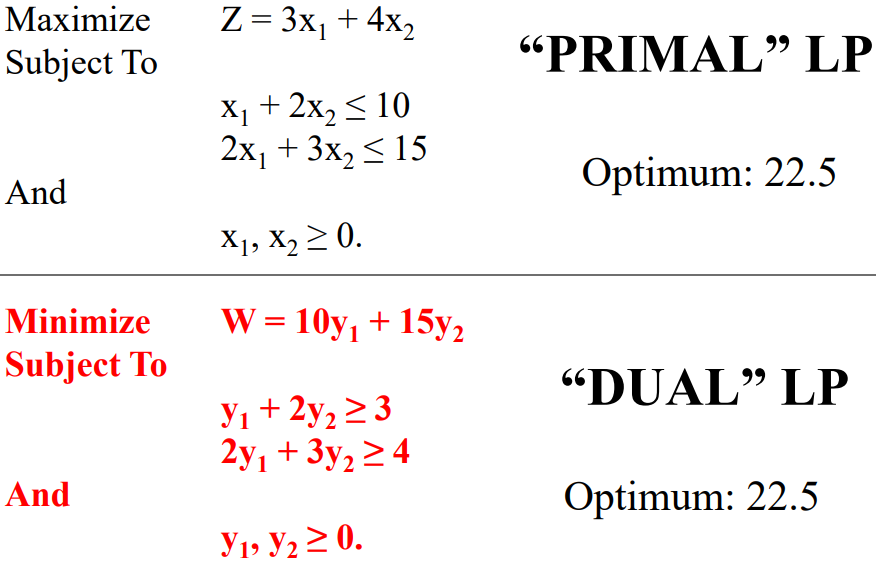
\includegraphics[scale=0.65]{images/lecture9_primalvsdual.PNG}
    \caption{Note that the LHS coefficients being the same for the dual LP is just a coincidence.}
\end{figure}

\newpage
\noindent
The \textbf{primal LP} is the one we have been constantly using so far, it is written in the form:
\begin{align*}
    &\mathrm{max} \quad Z = cx  \\[2pt]
    &\mathrm{s.t.} \quad 
    \begin{array}[t]{r c r}
        Ax & \leq & b \\
        x & \geq & 0
     \end{array}
\end{align*}

\noindent
The \textbf{dual LP} is closely related to the primal LP, and is written in the form:
\begin{align*}
    &\mathrm{min} \quad W = yb  \\[2pt]
    &\mathrm{s.t.} \quad 
    \begin{array}[t]{r c r}
        yA & \geq & c \\
        y & \geq & 0
     \end{array}
\end{align*}

\begin{figure}[h]
    \centering
    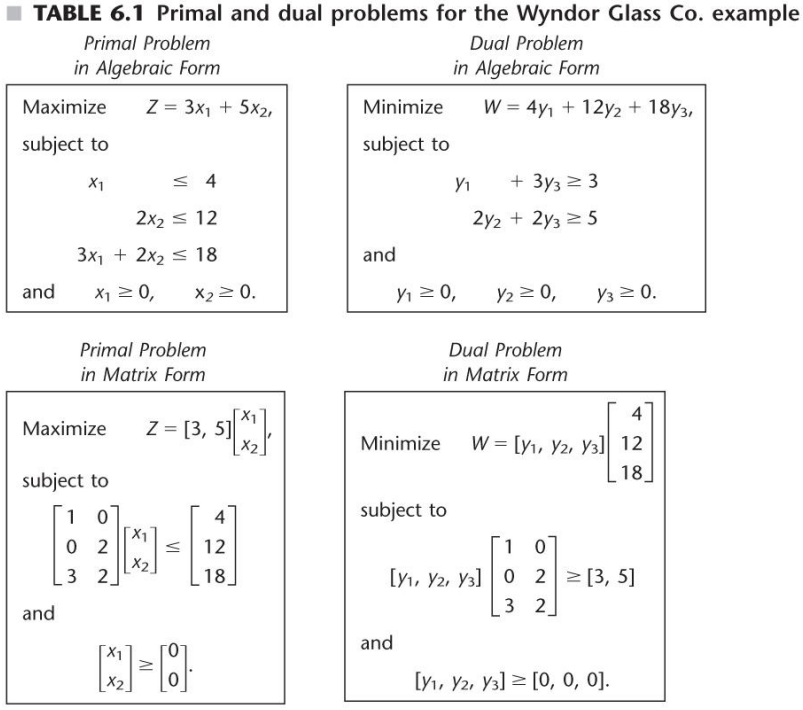
\includegraphics[scale=0.75]{images/lecture9_primaltodual.PNG}
\end{figure}

\noindent
In general, the following theorems describe the relation between the primal and dual LP:

\begin{itemize}
    \item \textbf{Weak Duality Theorem:} If $x$ is a feasible solution to the primal problem and $y$ is a feasible solution to the dual problem, then $cx \leq yb$ (this follows from the 'upper bound' intuition behind duality).
    \item \textbf{Strong Duality Theorem:} If $x^*$ is an optimal solution to the primal problem and $y^*$ is an optimal solution to the dual problem, then $cx^* = y^*b$ (they share the same optimum).
    \item The dual of the dual is the primal (all properties are symmetrical).
\end{itemize}

\newpage
\noindent
The full version of the \textbf{Strong Duality Theorem (SDT)} also takes into account the three possible states of an LP.
The SDT states that one of the following four situations holds:

\begin{enumerate}
    \item Both the primal and dual LP are feasible (i.e. they both have a finite optimum). This means for any optimal solution $x^*$ for the primal and $y^*$ for the dual $cx^* = y^*b$.
    \item The primal is \textit{infeasible}, and the dual is \textit{unbounded}.
    \item The primal is \textit{unbounded}, and the dual is \textit{infeasible}.
    \item Both LPs are infeasible.
\end{enumerate}

\noindent
If the primal has $m$ constraints and $n$ decision variables, the dual will have $n$ constraints and $m$ decision variables.
So if $m > n$, we can always choose to solve the dual instead.
This is what the \textbf{dual Simplex method} does.
It can be much quicker than the normal Simplex method, because the running time of the Simplex method is dominated by the number of functional constraints.

%
% Lecture 10
%
\section*{Lecture 10 - The SOB Method}
So far we showed how to construct the dual from a primal in the following standard form:

\begin{itemize}
    \item Maximization
    \item All constraints $\leq$
    \item All variables non-negative
\end{itemize}

\noindent
Note that when constructing a dual it is not necessary for the RHS to be non-negative.

\noindent
\\
How to construct the dual if the primal is not in standard form?
The easiest solution is first converting your program into standard form.
This is always possible because we don't care about the sign of the RHS:

\begin{figure}[h]
    \centering
    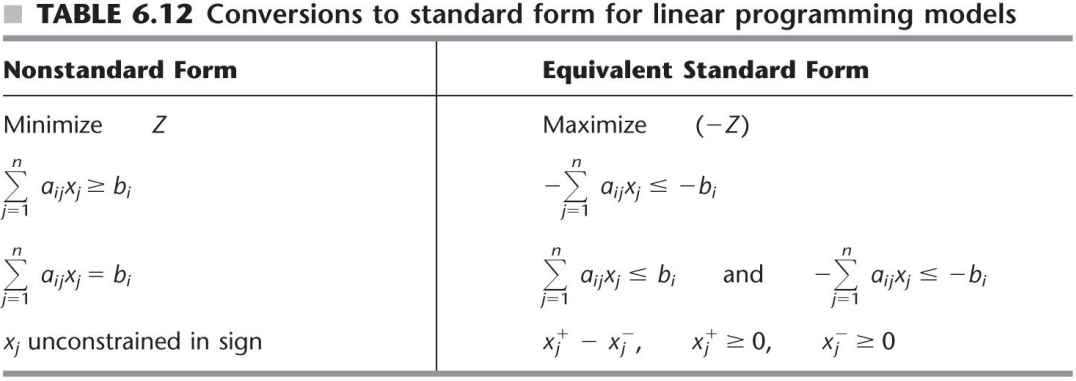
\includegraphics[scale=0.75]{images/lecture10_convertingtostandardform.PNG}
\end{figure}

\newpage
\noindent
There are, however, a few shortcuts for constructing the dual when the primal is not in standard form.
The advantage of these shortcuts is not only that they are faster, but they also produce a 'cleaner' dual with fewer variables and constraints.
One of these is the \textbf{Sensible, Odd, Bizarre Method (SOB)}:

\begin{figure}[h]
    \centering
    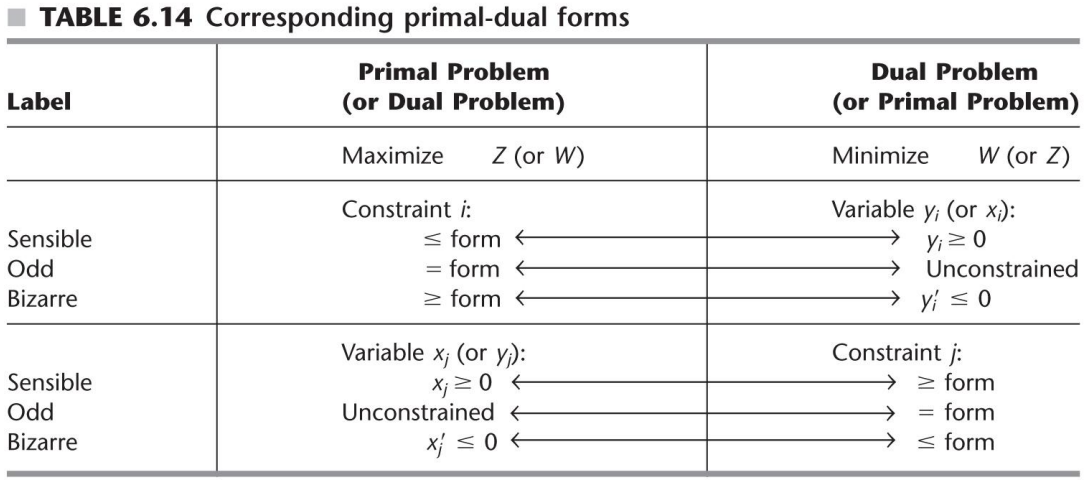
\includegraphics[scale=0.75]{images/lecture10_sobtable.PNG}
    \caption{This table will be given in the exam.}
\end{figure}

\noindent
Example:

\begin{figure}[h]
    \centering
    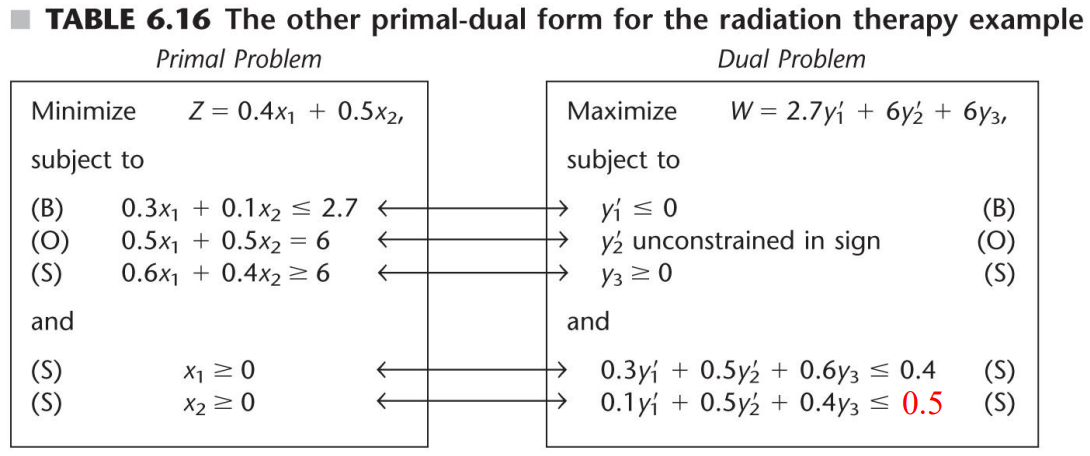
\includegraphics[scale=0.75]{images/lecture10_sobexample.PNG}
\end{figure}

%
% Lecture 11
%
\newpage
\section*{Lecture 11 - Simplex Duality}
First note that duality exists independently of any particular method for solving LPs (the dual always exists).
However, the Simplex method ties the primal and dual program together nicely in the following way:

\begin{figure}[h]
    \centering
    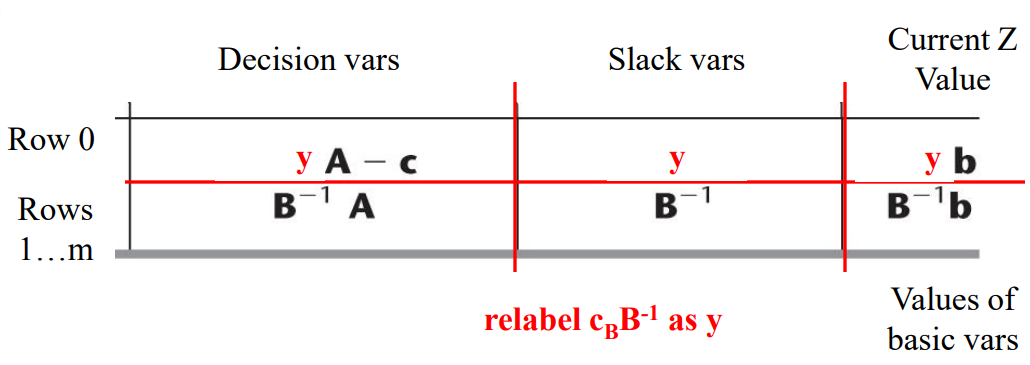
\includegraphics[scale=0.65]{images/lecture11_primaldualsimplexlink.PNG}
\end{figure}

\noindent
Compare this to how we write the dual:
\begin{align*}
    &\mathrm{min} \quad W = \textcolor{red}{yb}  \\[2pt]
    &\mathrm{s.t.} \quad 
    \begin{array}[t]{r c r}
        \textcolor{red}{yA - c} & \geq & 0 \\
        \textcolor{red}{y} & \geq & 0
     \end{array}
\end{align*}

\noindent
These values are in the top row of the Simplex tableau.

\noindent
\\
The top row of the Simplex tableau always encodes a complementary dual solution.
This complementary dual solution always has the same objective function value ($W = Z$), but most of the time the complementary dual solution will not be feasible.

\noindent
\\
Remember how a solution is optimal in the Simplex tableau if the top row has no negative values, and how a dual solution is feasible if all its values are non-negative.
This means \textbf{primal \underline{optimality} is equivalent to complementary dual \underline{feasibility}}.

\noindent
\\
Basically what the Simplex method does is maintain primal feasibility whilst trying to create dual feasibility as quickly as possible.
Since the dual is also a linear program, it also has basic solutions.
The complementary dual solution is also basic, but only becomes a basic \textit{feasible} solution when the primal solution is optimal.

\noindent
\\
Note that each basic solution in the primal LP has a complementary basic solution in the dual LP, where their respective objective functions are equal.
In these associated solutions, basic variables in the primal are nonbasic in the dual, and nonbasic variables in the primal are basic in the dual.

\newpage
\begin{figure}[h]
    \centering
    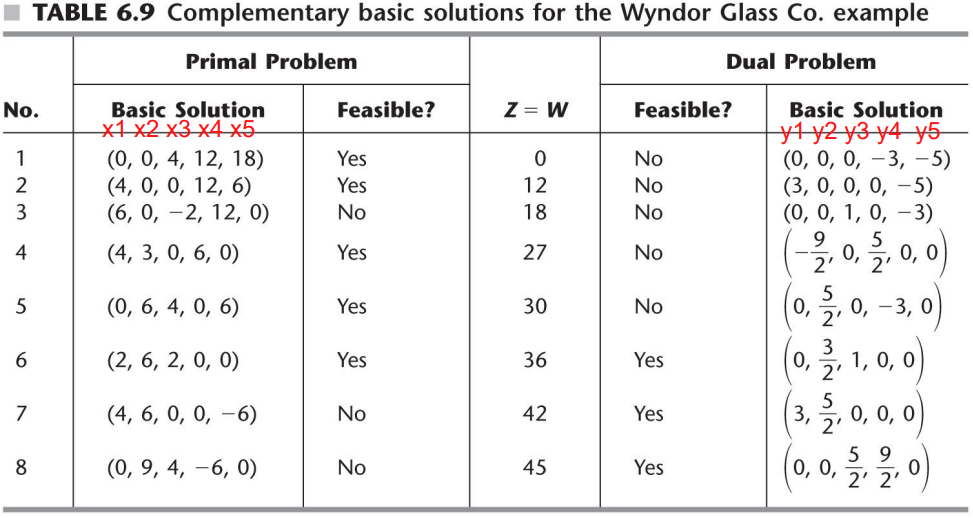
\includegraphics[scale=0.75]{images/lecture11_bfslink.PNG}
\end{figure}

\noindent
Basic solutions can be classified as one of the following (viewed from the primal):

\begin{itemize}
    \item \textbf{Optimal:} all basic variables are non-negative, top row is non-negative.
    \item \textbf{Suboptimal:} all basic variables are non-negative, at least one negative value in the top row.
    \item \textbf{Super-optimal:} at least one basic variable is negative, top row is non-negative.
    \item \textbf{Neither feasible nor super-optimal:} at least one basic variable is negative, at least one non-negative value in the top row.
\end{itemize}

\noindent
This relates the complementary basic solutions in the following way:

\begin{itemize}
    \item If both the primal and dual solutions are feasible, they are both \textbf{optimal}.
    \item If one of them is feasible and the other is infeasible, then the feasible one is \textbf{suboptimal}, and the infeasible one is \textbf{super-optimal}.
    \item If neither is feasible then \textbf{neither the primal nor dual is feasible or super-optimal}.
\end{itemize}

\noindent
See the table above for examples.

\subsection*{Complementary Slackness Theorem}
For each constraint in the primal or dual problem, either the constraint is satisfied with equality or the corresponding variable in the other problem is equal to 0.
In other words, if we pair a constraint in one problem with a variable in the other problem, then at most one of them can be non-zero.

%
% Lecture 12
%
\newpage
\section*{Lecture 12 - Primal-Dual Examples}
\subsection*{Example 1}
Given primal LP:
\begin{align*}
    &\mathrm{max} \quad 3x_1 + 5x_2  \\[2pt]
    &\mathrm{s.t.} \quad 
    \begin{array}[t]{r c r c r c r c r c r}
        x_1 & & & + & x_3 & & & & & = & 4 \\
        & & 2x_2 & & & + & x_4 & & & = & 12 \\
        3x_1 & + & 2x_2 & & & & & + & x_5 & = & 18
    \end{array}\\
    &\mathrm{and} \quad x_1, x_2, x_3, x_4, x_5 \geq 0
\end{align*}

\noindent
And corresponding dual LP:
\begin{align*}
    &\mathrm{min} \quad 4y_1 + 12y_2 + 18y_3  \\[2pt]
    &\mathrm{s.t.} \quad 
    \begin{array}[t]{r c r c r c r c r c r}
        y_1 & & & + & 3y_3 & - & y_4 & & & = & 3 \\
        & & 2x_2 & + & 2y_3 & & & - & y_5 & = & 5
    \end{array}\\
    &\mathrm{and} \quad y_1, y_2, y_3, y_4, y_5 \geq 0
\end{align*}

\noindent
Consider the following primal BFS:
\[ (x_1, x_2, x_3, x_4, x_5) = (4, 3, 0, 6, 0) \]

\noindent
Construct the complementary dual basic solution.
Is the above BFS optimal for the primal LP?
If not, what would be the entering basic variable if the Simplex method would continue pivoting. 

\subsection*{Solution 1}
We know $x_1, x_2$ and $x_4$ are basic variables.
The Simplex method ties the primal and dual problems together in the following way:
\[  (x_1, x_2, x_3, x_4, x_5) = (y_4, y_5, y_1, y_2, y_3) \]

\noindent
This means $y_4, y_5$ and $y_2$ are nonbasic variables.
To get the values of basic variables $y_1$ and $y_3$, plug them into the constraints of the dual LP and solve the resulting equations.
This gives the following complementary basic solution:
\[ (y_1, y_2, y_3, y_4, y_5) = (-4\frac{1}{2}, 0, 2\frac{1}{2}, 0, 0) \]

\noindent
The primal BFS is not optimal, because the complementary basic solution is not feasible ($y_1 < 0$).
The entering basic variable would be $x_3$, because that is the variable corresponding to the negative $y_1$.

\newpage
\subsection*{Example 2}
Given primal LP:
\begin{align*}
    &\mathrm{max} \quad 3x_1 - 8x_2 \\[2pt]
    &\mathrm{s.t.} \quad 
    \begin{array}[t]{r c r c r}
        x_1 & - & 2x_2 & \leq & 10
    \end{array}\\
    &\mathrm{and} \quad x_1, x_2 \geq 0
\end{align*}

\noindent
Construct the dual LP and find its optimum by inspection.
Use this optimum to find the optimum BFS of the primal LP.

\subsection*{Solution 2}
The dual LP is:
\begin{align*}
    &\mathrm{min} \quad 10y_1 \\[2pt]
    &\mathrm{s.t.} \quad 
    \begin{array}[t]{r c r}
        y_1 & \geq & 3 \\
        y_1 & \leq & 4
    \end{array}\\
    &\mathrm{and} \quad y_1 \geq 0
\end{align*}

\noindent
By inspection, the optimum solution to this LP is 30 ($y_1 = 3$).

\noindent
\\
To find the corresponding primal basis, first write both LPs in augmented form:
\[ x_1 - 2x_2 + x_3 = 10 \]

\[ y_1 - y_2 = 3 \]
\[ y_1 + y_3 = 4 \]

\noindent
We already know $(y_1, y_2, y_3) = (3, 0, 1)$.
This means $x_2$ and $x_3$ are nonbasic variables, and $x_1$ is a basic variable ($(x_1, x_2, x_3) = (y_2, y_3, y_1)$).
Plugging this into the primal constraint we get the optimum BFS of the primal LP:
\[ (x_1, x_2, x_3) = (10, 0, 0) \]

%
% Lecture 13
%
\newpage
\section*{Lecture 13 - Duality in Sensitivity Analysis}
After solving an LP, suppose someone asks you to re-solve the LP with slightly changed coefficients.
You could just re-solve it from the beginning, but this is really inefficient for large LP problems.
There are many changes that can be made to an LP, in this section we will focus on changes that don't disrupt the 0/1 pattern in the Simplex tableau.

\subsection*{Changing a nonbasic variable}
Suppose someone wants you to reanalyze your LP after changing some coefficients (either in $A$ or in $c$) of decision variable $x_k$, where $x_k$ is nonbasic in the current optimal solution.
We can ask ourselves the following questions:

\begin{itemize}
    \item \textbf{Is the old optimum still feasible?} The answer is yes. Since we do not touch any of the basic variables, our old solution is guaranteed to still be feasible.
    \item \textbf{Is the old optimum still optimal?} We can use the dual to check this. Modify the constraint corresponding to the variable we changed, plug in the values from the top row of the Simplex tableau, and check if the constraint is still satisfied.
\end{itemize}

\noindent
Say that, after applying the above step, the corresponding constraint looks something like $0.5 \geq 2$.
This means of course that the old optimum is no longer optimal, but also that this variable has a \textbf{surplus} of $-1.5$.
The new top row of the Simplex method will have $-1.5$ in the column corresponding to this variable.

\subsection*{Adding a new variable}
Suppose someone wants you to reanalyze your LP after adding a new variable $x_{new}$.
We can ask ourselves the following questions:

\begin{itemize}
    \item \textbf{Is the old optimum still feasible?} Assuming $x_{new}$ gets initialized with a value of 0 (i.e. nonbasic), the answer is yes. The LHS of the constraints remain unchanged.
    \item \textbf{Is the old optimum still optimal?} We can once again use the dual to check this. Creating a new primal variable corresponds to adding a new constraint to the dual LP. We can plug in the values from the top row of the Simplex tableau, and check if the new constraint is satisfied.
\end{itemize}

\subsection*{Re-optimization}
Sometimes an LP changes in a way such that the original optimum becomes \textbf{super optimal} (i.e. top row non-negative but infeasible / at least one basic variable becomes negative).
If this happens the BF solution is no longer primal-feasible, but the complementary dual solution \textit{is} still feasible.
In this situation we can re-calculate the new optimum by applying the Simplex method to the dual LP, using it as an 'advanced starting point'.

%
% Lecture 14
%
\newpage
\section*{Lecture 14 - Essence of Sensitivity Analysis}
Given $A, b, c$ and a basis we can obtain $B$ by taking the columns of $[A:I]$ corresponding to the basic variables.
With this, we can fully reconstruct the corresponding Simplex tableau.

\noindent
\\
Suppose we change our LP in the following way:
\[ A \rightarrow \bar{A} \text{ (changes to LHS)} \]
\[ b \rightarrow \bar{b} \text{ (changes to RHS)} \]
\[ c \rightarrow \bar{c} \text{ (changes to OBJ)} \]

\noindent
What happened to the previous optimal BF solution?
Is it still feasible?
Is it still optimal?
One way you could answer this is by resampling $B$ from scratch.
But for reconstructing the entire Simplex tableau you need $B^{-1}$, which for large LPs can take some time to compute.

\noindent
\\
In sensitivity analysis we express the changes to the LP as \textit{incremental changes} to the original coefficients.
To do this we can view $B^{-1}$ as an encoding of the set of elementary row operations we applied to get from the original tableau to the current tableau.
In summary, the algorithm works as follows:

\begin{enumerate}
    \item Record the final $B^{-1}$ and $c_B B^{-1}$ from the previous final tableau. Call them $S^*$ and $y^*$.
    \item Adjust the coefficients of the LP.
    \item Change the final tableau correspondingly (but keep $S^*$ and $y^*$ fixed!).
    \item If necessary, use Gaussian elimination to restore the 0/1 form of the tableau.
    \item Check feasibility (RHS non-negative?).
    \item Check optimality (top row non-negative?).
    \item If necessary, re-optimize from this starting point.
\end{enumerate}

\begin{figure}[h!]
    \centering
    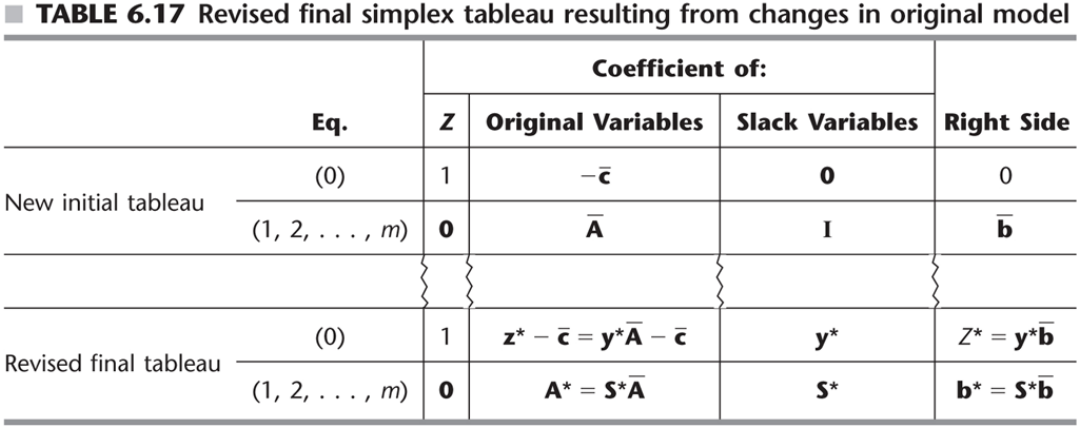
\includegraphics[scale=0.75]{images/lecture14_revisedsimplextableau.PNG}
\end{figure}

%
% Lecture 15
%
\newpage
\section*{Lecture 15 - Applying Sensitivity Analysis}
There are 4 'cases' in which sensitivity analysis can be applied.

\subsection*{Case 1: Changing the RHS ($b \rightarrow \bar{b}$)}
Because only $b$ changes, we won't have to apply any corrective Gaussian elimination.
We will also still be optimal, but we might lose feasibility if the RHS of the revised Simplex tableau (see table above) becomes negative.

\noindent
\\
Say we want to change one of the RHS values, what is the maximum increase or decrease we can apply without losing feasibility?
Assume all other RHS values remain untouched.
For this we can use \textbf{incremental analysis}:

\noindent
\\
Observe that $\bar{b} = b + \Delta b$.
This means $S^*\bar{b} = S^*b + S^*\Delta b = B^{-1}b + S^*\Delta b = $ old values of the basic variables + some change.
Say we have the following $b$ vector and $S^*$ matrix:
\[ b = \begin{pmatrix}
    2\\
    6\\
    2
\end{pmatrix}, S^* = \begin{bmatrix}
    1 & \frac{1}{3} & -\frac{1}{3}\\
    0 & \frac{1}{2} & 0\\
    0 & -\frac{1}{3} & \frac{1}{3}
\end{bmatrix} \]

\noindent
And we want to change the value of $b_2$.
Using the information given above, and the knowledge that the new RHS has to be non-negative to be feasible, we can write the following inequalities:
\begin{align*}
    0 \leq 2 + \frac{1}{3}\Delta b_2 \\
    0 \leq 6 + \frac{1}{2}\Delta b_2 \\
    0 \leq 2 - \frac{1}{3}\Delta b_2
\end{align*}

\noindent
Solving these leads to the inequalities $\Delta b_2 \geq -6$, $\Delta b_2 \geq -12$ and $\Delta b_2 \leq 6$.
This means we can \textit{increase} $b_2$ by at most 6 and \textit{decrease} it by at most 6.
This is also the "allowable range" in which the \textbf{shadow price} applies.

\noindent
\\
If we want to change multiple $b_i$ values at the same time, we can use the \textbf{100\% rule}:
\[ b = \begin{pmatrix}
    4\\
    12\\
    18
\end{pmatrix} \rightarrow \bar{b} = \begin{pmatrix}
    4\\
    15\\
    15
\end{pmatrix} \]

\noindent
Say $b_2$ and $b_3$ both have an allowed increase of 6 and an allowed decrease of 6.
The change in $b_2$ is $+3$, which is 50\% of the allowed increase.
The change in $b_3$ is $-3$, which is 50\% of the allowed decrease.
The total change is $50\% + 50\% = 100\%$.
This is $\leq 100\%$, so we can be sure that the old BFS remains feasible.
 
\newpage
\subsection*{Case 2a: Changing a nonbasic variable}
This is similar to lecture 13, but slightly more in depth.
Say we want to change the coefficients of a nonbasic variable $x_j$:
\[ A_j \rightarrow \bar{A}_j \]
\[ c_j \rightarrow \bar{c}_j \]

\noindent
The new tableau won't need any corrective Gaussian elimination, because we don't care about what is in the columns of nonbasic variables.
It will also still be feasible, because the values of the basic variables do not change.
We lose optimality if the value of $x_j$ in the top row goes negative, which we can detect using the dual like we discussed previously.

\noindent
\\
Suppose we \textit{only} want to change a coefficient $c_j$ (corresponding to nonbasic variable $x_j$).
Because this is a special subcase of what we just discussed, we know the only thing that can go wrong is that we lose optimality.
Say we want to know how far we can change $c_j$ without losing optimality.
Since we know that $c$ is the RHS of the dual, this reduces to case 1.

\subsection*{Case 2b: Introducing a new variable}
We pretend that the new variable has been there the entire time, with 0 as its coefficient everywhere in its column.
This reduces to case 2a.

\subsection*{Case 3: Changing a basic variable}
Say we want to change the coefficients of a basic variable $x_j$:
\[ A_j \rightarrow \bar{A}_j \]
\[ c_j \rightarrow \bar{c}_j \]

\noindent
The new tableau will require corrective Gaussian elimination \textit{most of the time}.
Until this has been done, it will not be clear whether the new solution will be feasible or optimal.

\noindent
\\
The only two things we need to compute are:
\[ y^* \bar{A}_j - \bar{c}_j \text{ (new coefficient in the top row)} \]
\[ S^* \bar{A}_j \text{ (rest of the column)} \]

\noindent
From here on we can apply Gaussian elimination to restore the 0/1 form of the $x_j$ column.
Once we have this tableau, we can apply standard methods to check feasibility and optimality.

\noindent
\\
There \textit{is} a risk that making changes to the coefficients of basic variable causes the columns of the basic variables in the final Simplex tableau to no longer be linearly independent.
This is a theoretical possibility that you should be aware of, but for this course that is all you need to know.

\newpage
\noindent
We know what to do when we change the objective function coefficient of nonbasic variables: work out the maximum / minimum change such that the coefficient of $x_j$ in the top row remains non-negative.
If we want to do this for basic variables, we need to take the Gaussian elimination steps into account.

\noindent
\\
Say we increment $c_j$ by $\Delta c_j$.
The coefficient of the top row for column $j$ becomes $y^* \bar{A}_j - \bar{c}_j = y^* \bar{A}_j - (c_j + \Delta c_j) = -\Delta c_j$.
The next step is to set this coefficient to 0 again using Gaussian elimination.
For example, given matrix:
\[ \begin{bmatrix}
    0 & -\Delta c_2 & \frac{3}{4} & 0 & \frac{3}{4}\\
    1 & 0 & 1 & 0 & 0\\
    0 & 1 & -\frac{3}{4} & 0 & \frac{1}{4}\\
    0 & 0 & \frac{9}{4} & 1 & -\frac{3}{4}
\end{bmatrix} \]

\noindent
We can transform the top row into:
\[ \begin{bmatrix}
    0 & 0 & \frac{3}{4} - \frac{3}{4}\Delta c_2 & 0 & \frac{3}{4} + \frac{1}{4}\Delta c_2
\end{bmatrix} \]

\noindent
We can apply the strategy discussed in case 2a to this top row to find the maximum and minimum range of $c_j$.

\subsection*{Case 4: Introducing a new constraint}
How do you determine whether the previous optimal BFS is still feasible?
Just evaluate the new constraint at the old BFS (this is similar to case 2b, except here we evaluate a new primal constraint).
If the old BFS is still feasible, it is also still optimal (because the new LP is more constraint than the old one, the optimum cannot possibly increase).

\noindent
\\
If we lost feasibility, we need to adjust the Simplex tableau.
We can obtain the new Simplex tableau as follows:

\begin{enumerate}
    \item Allocate a new slack variable to the constraint.
    \item Take the initial row of the Simplex tableau that you would have used for this constraint.
    \item Add this row to the final Simplex tableau.
    \item Apply Gaussian elimination correction if necessary.
    \item Re-optimize if necessary.
\end{enumerate}

\noindent
Some large LPs have a huge number of constraints, far more than necessary.
An alternative way to solve these LPs is to add constraints one at a time, only if needed.
This technique is also often applied when solving LP-relaxations of ILP problems.
A similar idea can be applied to the dual, where it is called "column generation".

\end{document}
